% Author: David Paulino
% Date: 2023-03-03
% Description: LaTeX Template


\documentclass[12pt]{article}

% Document en français
\usepackage[french]{babel}

\usepackage[utf8]{inputenc}
\usepackage[T1]{fontenc}
\usepackage{graphicx}
\usepackage{amsmath}
\usepackage{amssymb}
\usepackage{amsthm}
\usepackage{amsfonts}
\usepackage{amscd}
\usepackage{amstext}

\usepackage{hyperref}
\usepackage{xcolor}
\usepackage{fancyhdr}
\usepackage{setspace}
\usepackage{float}
\usepackage{subfig}
\usepackage{caption}
\usepackage{listings}
\usepackage{tikz}
\usepackage{pgfplots}
\usepackage{pgfplotstable}
\usepackage{pgf}

% Add references in table of contents
\usepackage[nottoc]{tocbibind}

% Set author and place
\newcommand{\DP}{David Paulino}
\newcommand{\place}{Genève}
\newcommand{\fulltitle}{Analyse et optimisation de l'expected goal: application au machine learning}
\newcommand{\shorttitle}{Analyse et optimisation de l'expected goal}

% On retire l'indentation des paragraphes
\setlength{\parindent}{0pt}
% Augmentation de l'espacement entre les sauts de ligne
%\setlength{\parskip}{5pt} % Modifier la valeur selon vos besoins

% Title
\title{\fulltitle}
\author{\DP}
\date{\today}

% Header
\pagestyle{fancy}
\fancyhf{}
\renewcommand{\headrulewidth}{0pt}
\lhead{\DP}
\rhead{\shorttitle}

% Footers
\lfoot{Page \thepage}
\rfoot{\today}

% Document
\begin{document}

% Title page
\begin{titlepage}

    \begin{figure}[h]
        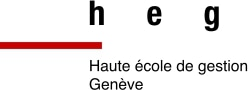
\includegraphics[width=0.3\textwidth]{img/logo_heg-ge.jpg}
    \end{figure}

    \vspace*{0.5cm}

    \begin{center}

        \begingroup \linespread{1,75} \selectfont
        {\Large \fulltitle}\\[0,75cm]
        \endgroup


        % Make a vertical space

        \vspace{1.5cm}

        \textsc{\large Travail de Bachelor HES réalisé en vue de \newline l’obtention du Bachelor par :}\\[0,50cm]

        \begingroup \linespread{1,5} \selectfont
        \textsc{\large \DP}\\[0,50cm]
        \endgroup


        \vspace{1cm}


        \textsc{\large Conseillers au travail de Bachelor : }

        \begingroup \linespread{1,5} \selectfont
        \textsc{\large Pr Alexandros KALOUSIS}\\[0.1cm]
        \textsc{\large Dr Nils SCHÄTTI}\\[1cm]
        \endgroup


        \begingroup \linespread{1,75} \selectfont
        \textsc{\large \place, le \today}\\[0,1cm]

        {\large Haute école de Gestion de Genève (HEG-GE)}\\[0,1cm]

        {\large Filière Informatique de gestion}\\[0,1cm]
        \endgroup



        \begin{figure}[h]
            \vspace{0.05cm}
            \hspace*{12cm}
\includegraphics[width=0.25\textwidth]{img/logo_hes-so.jpg}
        \end{figure}

    \end{center}



    \vfill
\end{titlepage}




\newpage

\section{Déclaration}
Ce travail de Bachelor est réalisé dans le cadre de l'examen final de la Haute école de gestion de Genève, en vue de l'obtention du titre de Bachelor of Science HES-SO en Informatique de gestion.
\newline\newline
L'étudiant a envoyé ce document par email à l'adresse remise par son conseiller au travail de Bachelor pour analyse par le logiciel de détection de plagiat URKUND, selon la procédure détaillée à l'URL suivante : \url{https://www.urkund.com}
\newline\newline
L'étudiant accepte, le cas échéant, la clause de confidentialité. 
L'utilisation des conclusions et recommendations formulées dans le travail de Bachelor, sans préjuger de leur valeur, n'engage ni la responsabilité de l'auteur, ni celle du conseiller au travail de Bachelor, du juré et de la HEG.
\newline\newline
"J'atteste avoir réalisé seul le présent travail, sans avoir utilisé des sources autres que celles citées dans la bibliographie."
% Faire un grand saut de ligne
\vspace{4cm}
% Aligner le texte à droite
\begin{flushright}
    Fait à \place, le \today
\end{flushright}

\begin{flushright}
    \DP
\end{flushright}
\vspace{1cm}
\begin{flushright}
    --------------------------------
\end{flushright}


\newpage

\section{Remerciements}
% Insérer les remerciements ici

J'aimerais tout d'abord remercier mon conseiller au travail de Bachelor, le docteur Nils Schätti pour son aide et ses conseils tout au long de ce travail. 
Ses remarques et son investissement ont été très utiles pour améliorer la qualité de cette thèse. 
\newline\newline
Je remercie également mon deuxième conseiller au travail de Bachelor, le professeur Alexandros Kalousis pour l'apport de ses idées et ses explications sur les concepts de machine learning.
\newline\newline
Je remercie également mon ami Rayane Ammad ainsi que ma belle-soeur, Alessia Marques, pour leur relecture et leurs retours sur ce travail.
\newline\newline
Finalement, je remercie ma famille pour leur soutien et leur patience tout au long de ma formation, spécialement mon père et ma mère.

\newpage

\section{Résumé}
% Insérer le résumé ici
Ce travail a pour but d'analyser et d'optimiser l'expected goal (xG) dans le football.
On cherche à comprendre comment est calculé l'expected goal, quelles sont ses variables les plus influentes et quels sont les modèles les plus performants pour établir un xG.
\newline\newline
Ce travail passe par plusieurs phases :
\begin{itemize}
    \item Une phase de recherche pour comprendre le fonctionnement du xG et les modèles existants
    \item Une phase de préparation des données pour les modèles
    \item Une phase de modélisation pour trouver le modèle le plus performant
    \item Une phase d'analyse des résultats
\end{itemize}


\newpage

% Liste des tableaux
\listoftables

\newpage

% Liste des figures
\listoffigures

\newpage

% Table of contents
\tableofcontents
\newpage

% Content
\section{Introduction}

% Citation avec Zotero et BibLaTeX
\subsection{Introduction à la problématique}
Lorsque les premiers sports sont apparus, l'information la plus importante était le score et le vainqueur de la confrontation.
Au fur et à mesure, plus d'informations sur les matchs sont venues s'ajoutées.
Le nombre de tirs dans un matchs par équipes, le nombre de passes, le nombre de tirs cadrés, la possession du ballon, le pourcentage de passes réussies, le nombre de passes décisives et d'autres sont venus s'ajouter aux statistiques dans le football.
Le pourcentage de réussite aux lancers francs, le nombre de rebonds, le nombre de passes décisives, le pourcentage de réussite aux tirs, le nombre de fautes, le nombre de minutes jouées, le pourcentage de réussite à 3 points et d'autres sont venus s'ajouter aux statistiques dans le basketball.
Ces statistiques sont également devenus personnelles à chacun des joueurs.
Nous pouvons également compter, pour le baseball, le nombre de fois qu'un joueur était au bâton, son nombre de double, de triples, son nombre de buts et bien d'autres.
\newline\newline
C'est d'ailleurs dans le baseball que nous retrouvons la première utilisation de statistiques avancées pour établir des stratégies.
En effet, au début des années 1970, un joueur des Baltimore Orioles a développé une analyse statistique pour choisir le meilleur alignement possible pour son équipe de départ.
Il s'agit de Davey Johnson.
Cependant, il n'a pas pu l'utiliser à ce moment-là puisque le président de sa franchise n'avait pas confiance. C'est qu'à partir de 1984 où il fut le coach des New York Mets qu'il a pu mettre en place son analyse statistique avancée pour établir le meilleur choix pour son équipe de départ. \cite{incPCMag1984}
Deux saisons plus tard, il remporte la Série mondiale 1986 \footnote{En MLB, la Série mondiale est la série finale qui permet de déterminer qui est l'équipe championne de la ligue.}. Les Mets étaient situés à la dernière place de leur conférence avant l'arrivée de Davey Johnson et son management orienté sur les statistiques.
\newline
Après cette réussite, les autres franchises de la MLB\footnote{Ligue majeure de baseball} ont également commencé à adopter l'analyse de statistiques dans le sport et cela a également été populaire dans les autres sports avec par exemple Daryl Morey qui a été le premier coach analyste statistiques recruté chez les Rockets de Houston en NBA en 2007. \cite{DarylMorey13year2020}
Les franchises de la NBA\footnote{Ligue nationale de basketball} ont par la suite également adopté une approche managériale statistique.
Nous constatons alors que cette culture de la statistique dans le sport provient des États-Unis.
\newline
Il est désormais important d'amener l'arrivée des expected goals. 
L'une des premières études sur un modèle d'expected goals vient d'Alan Ryder qui a publié une étude sur la qualité des tirs effectuées dans des matchs de hockey. \cite{ryderIsolatingShotQuality2004}
Ce dernier a pu analyser les différentes circonstances lors d'un tir et développer un modèle qui prédit la probabilité d'un tir selon les circonstances de celui-ci.
Dans le football, l'une des premieres études sur l'expected goal vient de Richard Pollard, Jake Ensum et Samuel Taylor ayant analysé les facteurs qui influent la chance de marquer un but. \cite{pollardEstimatingProbabilityShot2004} La problématique de ce travail est donc de pouvoir analyser et optimiser l'expected goal.
\newline\newline
Il semble maintenant important de savoir ce qu'est l'expected goal, qui est très souvent réduit par le terme "xG". 
Il est une métrique qui permet de déterminer la probabilité qu'un tir soit transformé en but selon les données de ce tir \cite{XGExplainedFBrefa}.
Ce dernier ayant un xG de 0.4 a une probabilité de 40\% d'être transformé en but. Un autre avec un xG à 1, qui est la plus grande valeur possible, aurait donc 100\% de chance d'être transformé en but.
\footnote{Il est important d'indiquer qu'il est très rare qu'un xG d'un tir soit égal à 1 mais il va généralement s'en rapprocher fortement selon ses paramètres.} \cite{pettyWhatExpectedGoals2018a}
\newline\newline
Pour comprendre ce qu'est réellement un xG, nous allons l'observer avec l'emplacement des tirs sur le terrains.
Sur la figure \ref{fig:shotmap}, nous pouvons voir un exemple d'emplacement de tirs et de leur xG.
\newline \newline
Par ailleurs, les xG se sont tellement développés que des métriques dérivées ont été créées. 
Nous pouvons, par exemple, citer le xA, qui est l'expected assist.
C'est une métrique qui permet de déterminer la probabilité qu'une passe soit transformée en passe décisive selon les données de cette passe. \cite{XGExplainedFBrefa}
Il existe également les xGA, qui sont les expected goals against. 
Ceux-ci permettent de déterminer la probabilité qu'un tir soit transformé en but selon les données de ce tir mais pour l'équipe adverse. \cite{pettyWhatExpectedGoals2018a}

Il y en a également d'autres comme les expected points qui sont les points qu'une équipe devrait avoir gagnés, ceci basé sur les données relatives aux xG. D'autres dérivés sont indiquées sur l'article de Pinnacle écrit par Luke Petty. \cite{pettyWhatExpectedGoals2018a}
\newline\newline
Maintenant que nous avons vu ce qu'est un xG et ces dérivés actuels, il semble pertinent de décrire l'utilisation de cette métrique dans le football actuel.

\begin{figure}[htp]
    \centering
    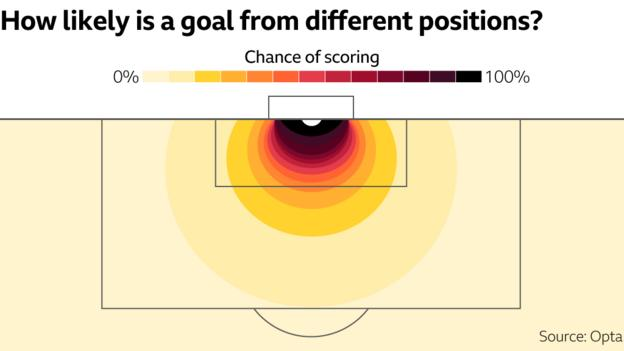
\includegraphics[width=0.8\textwidth]{img/SchemaXG.jpeg}

    \caption{Schéma montrant les chances de buts selon les positions des tirs - Source : Opta}
    \label{fig:shotmap}
\end{figure}
\subsection{Intérêt de la problématique}
Cette problématique est très intéressante puisque cette métrique représente une donnée dernièrement très populaire dans le monde du football. Elle donne plus d'informations sur le match que les autres statistiques d'un match (possession, nombre de passes, nombre de tirs cadrés, nombre de buts, etc.). 
Prenons comme example la possession de balle, une équipe peut en avoir 70\% pendant le match mais ne pas marquer de buts, ni même être dangereuse avec le ballon. 
Les tirs cadrés, s'ils sont tous effectués à l'extérieur de la surface de réparation, ne sont pas forcément dangereux. 
L'expected goal permet de donner une valeur à chaque tir et de déterminer si celui-ci a une chance d'être transformé en but.
\newline \newline
Certaines personnes utilisent cette métrique pour leurs paris sportifs. 
Ils observent la métrique lors des derniers matchs et la compare avec le score réel du match. 
Si la différence est grande, cela peut permettre de constater un manque de réalisme ou un sur-régime d'une des deux équipes. \cite{tennerelBienUtiliserExpected2022a}
\newline \newline
Les analystes utilisent cette donnée pour analyser les performances de leurs joueurs et de leurs équipes. Par exemple, la comparaison des xG et du nombre de buts marqués d'un joueur sur une période donnée peut permettre de déterminer la dangerosité et la capacité d'un buteur à terminer des actions. \cite{pettyWhatExpectedGoals2018a}
Les xG peuvent aussi être utilisés pour analyser les performances d'une équipe dans des situations bien précises. Une équipe qui possède un haut xG sur des contre-attaques montre qu'elle est très dangereuse sur ce type de situation. \cite{XGExplainedFBrefa}
L'une des choses les plus intéressante de cette métrique est qu'elle peut être utilisée pour analyser les forces et faiblesses des équipes. Par exemple, une équipe peut observer que ses xG sont très faibles lorsqu'elle tente des centres. Cela peut lui permettre de trouver son identité de jeu et de décider d'abandonner cette stratégie. Cette métrique est tout autant valable pour analyser les forces et faiblesses d'une équipe adverse. 
Dans la même situation, si une équipe vient à affronter une équipe qui a dû mal à produire des xG sur des centres, elle peut décider de la forcer à jouer sur des centres en libérant de l'espace sur les côtés par exemple.
\newline \newline
Cette métrique est également utilisée pour aider les recruteurs à juger les performances de finition d'un joueur \cite{garratt-stanleyWhatExpectedGoals2022}. Nous avons vu précédemment qu'il existait des dérivés des xG comme les xA\footnote{Passes décisives attendues}. 
Les différents dérivés peuvent permettre de juger les performances et qualités d'un joueur qui se trouve à un poste bien précis. 
Par exemple, un milieu de terrain ou un défenseur peut être jugé sur ses xA et un attaquant sur ses xG.


\subsection{Questions auquelles nous souhaitons répondre dans ce travail}
Il y a deux grandes questions à répondre dans ce travail.
\begin{itemize}
    \item Quels sont les paramètres qui influencent le plus l'expected goal ?
    \item Quel est le meilleur modèle pour prédire l'expected goal ?
\end{itemize}

Le but de ce travail est de comprendre quelles sont les variables qui influencent le plus les xG.
Cela permettra de comprendre quelles sont les variables les plus importantes pour prédire ces estimations de buts.
Grâce à cela, il est possible pour un analyste de données d'une équipe de football de savoir quelles sont les facteurs qui influencent le plus la qualité d'un tir.
Cela peut permettre de déterminer les forces et faiblesses d'une équipe et de savoir sur quels aspects travailler pour améliorer les performances de l'équipe.
\newline \newline
Le deuxième objectif de ce travail est de trouver le meilleur modèle pour prédire les xG.
En effet, le but sera d'avoir le modèle le plus performant et de comparer les différents modèles qui peuvent être utilisée pour établir cette métrique.
Il faut également veiller à ce que le modèle ne fasse pas de sur-apprentissage. Il est donc important de faire attention à la complexité du modèle et de trouver le meilleur compromis entre la complexité et la performance du modèle.

\newpage
\subsection{Plan du document}
Concernant le déroulement de ce travail, il y a plusieurs étapes.
Tout d'abord, il y a la recherche des travaux existants sur le sujet.
Cette étape est effectuée dans la section \ref{sec:synthese}.
Parmi ceux-ci, nous chercherons à savoir quels datasets ont été utilisés ainsi que les résultats obtenus.
Cela nous permettra de comparer nos résultats avec ceux obtenus dans les autres travaux et ainsi savoir si les résultats sont cohérents par rapport à l'état de l'art actuel des recherches scientifiques.
\newline \newline
La suite sera de trouver un dataset avec les informations nécessaires pour implémenter le modèle.
Cette étape de la thèse est très importante puisque c'est la base de notre recherche.
Une fois ce dataset trouvé, il va falloir le documenter. En effet, il est important de comprendre ce que chaque attribut représente.
L'étape suivante est importante pour visualiser les données.
Cela permettra de voir si les données sont exploitables et cohérentes.
Cela pourra également nous indiquer si des biais seront présents dans le modèle.
Cette section d'analyse du dataset est trouvable dans la section \ref{sec:dataset}.
\newline \newline
Une fois les données documentées et visualisées, il va falloir les préparer.
En effet, il pourrait y avoir des données manquantes mais qui sont disponibles après un traitement.
Il pourrait également y avoir des données qui ne sont pas exploitables et qui doivent être supprimées.
Par exemple, l'identifiant de la base de données d'un tir pourrait être supprimé car il n'apporte rien pour la prédiction de l'expected goal.
Cette section de transformation du dataset est également trouvable dans la section \ref{sec:dataset} qui fait suite à la section d'analyse du dataset initial.
\newline \newline
Ensuite, nous pourrons commencer à implémenter le modèle et observer les facteurs qui influencent la prédiction du xG.
Cette partie est trouvable dans la section \ref{sec:methodologie}.
C'est également à ce moment-là qu'il faudra comparer les différents modèles pour voir lequel est le plus performant pour prédire les xG.
La comparaison est trouvable dans la section \ref{sec:results} qui visent à montrer la fiabilité et la cohérence du modèle par rapport à la problématique initial.

\newpage
\section{Synthèse des travaux existants}
\label{sec:synthese}
Le premier travail repertorié sur les xG et la qualité d'un tir est celui de Richard Pollard, Jake Ensum et Samuel Taylor \cite{pollardEstimatingProbabilityShot2004}.
Dans ce dernier datant de 2004, la seule information indiquée concernant le dataset est que les données proviennent de la Coupe du monde 1986 et de celle de 2002.
Le modèle a été implémenté en utilisant une régression logistique.
Le nombre de tirs répertoriés dans ce travail est de 1096.
La conclusion de ce travail est que les 3 facteurs les plus influents pour la prédiction des xG sont :
\begin{itemize}
    \item La distance entre le tireur et le but
    \item L'angle du but en fonction de la position du tir
    \item L'espace entre le tireur et le défenseur le plus proche
\end{itemize}
Le résultat final de l'analyse de la régression logistique de ce travail ressemble à cela.
\begin{table}[htp]
    \centering
    \begin{tabular}{|l|l|l|l|l|l|l|}
        \hline
        \textbf{Predictor} & \textbf{Coefficient} & \textbf{z} & \textbf{p} & \textbf{ratio} & \textbf{Lower} & \textbf{Upper} \\ \hline
        Constant           & 0.3771               & 1.20       & 0.229      &                &                &                \\ \hline
        Distance           & -0.1586              & -9.51      & 0.000      & 0.85           & 0.83           & 0.88           \\ \hline
        Angle              & -0.0222              & -3.81      & 0.000      & 0.98           & 0.97           & 0.99           \\ \hline
        Space              & 0.7991               & 3.22       & 0.001      & 2.22           & 1.37           & 3.62           \\ \hline
    \end{tabular}
    \caption{Résultats de la régression logistique du travail de Pollard, Ensum et Taylor}
\end{table}

Le deuxième travail est celui de Izzatul Umami, Deden Hardan Gutama et Heliza Rahmania Hatta \cite{umamiImplementingExpectedGoal2021}. 
Il utilise les données de Wyscout des 5 championnats majeurs en Europe de la saison 2019-20. 
Les auteurs ont décidés de prendre comme données :
\begin{itemize}
    \item La distance
    \item L'angle
    \item Si le tir est un tir de la tête ou pas
\end{itemize}
Dans le dataset, 32000 tirs ont été utilisés pour la création du modèle.
Comme pour le travail précédent, la régression logistique a été utilisée.
Il est également indiqué qu'une séparation du dataset a été faite pour avoir des données d'entraînement et de test.
Dans leurs tests du modèle, il est indiqué que le but est de faire de la classification pour de futures instances, il faut donc utiliser un seuil.
Suite à l'utilisation de ce dernier pour la classification, une matrice de confusion a été faite pour ensuite calculer la spécificité et la sensibilité du modèle.
Ce principe de sensibilité et spécificité permet de choisir la meilleure performance selon le contexte d'utilisation du modèle.
\begin{equation}
    Sensitivity = \frac{True Positive}{True Positive + False Negative}
\end{equation}
\begin{equation}
    Specificity = \frac{True Negative}{True Negative + False Positive}
\end{equation}
Pour calculer la sensibilité et la spécificité, nous pouvons voir que nous avons besoin des "True Positive", "True Negative", "False Positive" et "False Negative".
Les "True Positive" sont les tirs qui sont des buts ayant été correctement prédits et les "True Negative" sont les tirs qui sont manqués ayant été également correctement prédits.
À l'inverse, les "False Positive" sont les tirs qui ont été manqués ayant été prédits comme des buts et de même pour les "False Negative" qui sont des tirs qui sont des buts ayant été prédits comme des tirs manqués.
La valeur de chacune de ces variables est donc le nombre d'instances correspondant à la description.
\newline \newline
La sensibilité permet de voir la capacité du modèle à prédire correctement les tirs qui seront des buts.
De l'autre côté, la spécificité permet de voir la capacité du modèle à prédire correctement les tirs qui ne seront pas des buts.
Comme indiqué dans le travail de Umami, Gutama et Hatta, la spécificité est plus importante que la sensibilité selon le contexte.
Dans le cas où le modèle est utilisé pour prédire un cancer, nous allons chercher à avoir une meilleur sensibilité pour éviter de passer à côté d'un cancer. \cite{umamiImplementingExpectedGoal2021}
Cela leur permet de savoir comment choisir le seuil pour la classification.
En conclusion de leur travail, ils ont obtenu une sensibilité de 0.9672 et une spécificité de 0.1903 pour un seuil 0.02.
Ils indiquent finalement que le modèle de xG est plus performant si nous prenons la distance et l'angle en compte plutôt que de prendre uniquement la distance.
\newline\newline
Un travail qui fournit également du code est celui de David Sumpter \cite{sumpterFittingXGModel}. 
Son objectif est de créer un modèle de xG en utilisant une régression logistique. 
Il utilise les données de Wyscout du championnat anglais de la saison 2017-18. 
David Sumpter explique étape par étape ce qui est effectué pour créer et améliorer son modèle.
Il y a également des pistes pour convertir les positions X et Y en distance et en angle.
Il commence par créer un modèle de xG en utilisant uniquement la distance. 
Par la suite, il le fait uniquement avec l'angle.
Finalement, il utilise de multiples facteurs, comme la distance au carré ou encore l'angle multiplié par la position X du tir, pour créer son modèle et produit un résumé de la régression logistique.

\begin{table}[htp]
    \centering
    \begin{tabular}{|l|l|l|l|l|l|l|}
    \hline
    \textbf{Predictor} & \textbf{coef} & \textbf{std err} & \textbf{z} & \textbf{P\textgreater{}|z|} & \textbf{{[}0.025} & \textbf{0.975{]}} \\ \hline
    Intercept          & -0.5103       & 0.887            & -0.576     & 0.565                       & -2.248            & 1.228             \\ \hline
    Angle              & -0.6338       & 0.319            & -1.989     & 0.047                       & -1.258            & -0.009            \\ \hline
    Distance           & 0.2798        & 0.118            & 2.381      & 0.017                       & 0.049             & 0.510             \\ \hline
    X                  & -0.1243       & 0.124            & -1.001     & 0.317                       & -0.368            & 0.119             \\ \hline
    C                  & 0.0300        & 0.040            & 0.750      & 0.454                       & -0.048            & 0.109             \\ \hline
    X2                 & -0.0014       & 0.001            & -1.422     & 0.155                       & -0.003            & 0.001             \\ \hline
    C2                 & -0.0041       & 0.003            & -1.398     & 0.162                       & -0.010            & 0.002             \\ \hline
    AX                 & 0.1251        & 0.118            & 1.063      & 0.288                       & -0.105            & 0.356             \\ \hline
    \end{tabular}
    \caption{Résumé de la régression logistique du modèle de xG de David Sumpter}
\end{table}
Il n'y a pas moyen de connaître les coefficients uniquement pour la distance et l'angle car aucun résumé n'est fait pour ces deux facteurs uniquement.
\newline\newline
Le dernier travail est fait par H.P.H Eggels. 
Le but est d'expliquer le résultat d'un match en utilisant les xG. 
Dans ce travail, il utilise un modèle de xG pour prédire le résultat d'un match.
Les données du travail proviennent de ORTEC, de Immotio et FIFA. En effet, son article scientifique utilise trois datasets pour créer son modèle de xG. \cite{eggelsExpectedGoalsSoccer2016}.
Il y a eu un travail de "merging" des données pour avoir un dataset qui contient toutes les informations nécessaires pour créer le modèle. 
Cependant, les datasets peuvent avoir des problèmes entre eux lors du "merging". 
Par exemple, les noms des joueurs qui sont différents (majuscule, accent, encodage, surnom, etc.) a été un problème mais une solution a été trouvée.
\newline
Le dataset utilisé contient donc trois sources de données différentes (voir tab. \ref{tab:data_from_eggels}).
\begin{table}[htp]
    \centering
    \begin{tabular}{lll}
    \hline
    \textbf{ORTEC}  & \textbf{FIFA}       & \textbf{Immotio}                  \\ \hline
    Context         & Player quality      & Number of attackers in line       \\
    Part of body    & Goal keeper quality & Number of defenders in line       \\
    Dist to goal    &                     & Distance nearest defender in line \\
    Angle to goal   &                     & Distance goal keeper              \\
    Originates from &                     &                                   \\
    Current score   &                     &                                   \\
    High            &                     &                                   \\ \hline
    \end{tabular}
    \caption{Sources de données utilisées par H.P.H Eggels}
    \label{tab:data_from_eggels}
\end{table}
\newpage
Parmi les modèles testés, ce travail utilise :
\begin{itemize}
    \item Un modèle de régression logistique
    \item Random Forest
    \item Un arbre de décision
    \item Ada-boost
\end{itemize}
Pour chacun de ces modèles, il y a une liste des différents paramètres qui vont être utilisés pour trouver le meilleur d'entre eux.
Chacun des modèles a suivi une procédure avec un set d'entraînement, un set de validation et un set de test.
Le set de validation permet de trouver les meilleurs paramètres pour le modèle.
Le set de test permet de tester le modèle avec les paramètres trouvés et le comparer avec les autres modèles
Le modèle le plus performant parmi les quatres cités est le Random Forest avec une précision de 0.771.
Cependant, il n'est pas possible de connaître les meilleurs hyper paramètres pour chacun des modèles.
Ce travail donne tout de même de bonnes pistes pour l'ajout de nouvelle données pour améliorer le modèle de xG.
\newpage

\subsection{Récapitulatif des travaux existants}
\begin{table}[htp]
    \centering
    \begin{tabular}{lll}
    \hline
    \textbf{Auteur(s)}                                                                                   & \textbf{Source de données}                                                                               & \textbf{Conclusion}                                                                                                                                          \\ \hline
    \begin{tabular}[c]{@{}l@{}}Richard Pollard\\ Jake Ensum\\ Samuel Taylor\end{tabular}                 & \begin{tabular}[c]{@{}l@{}}Coupe du monde \\ 1986 et 2002\end{tabular}                                   & \begin{tabular}[c]{@{}l@{}}La distance, l'angle \\ et l'espace avec le \\ joueur le plus proche \\sont les variables \\qui ont le plus d'influences \\sur l'estimation de but\end{tabular}                                                 \\ \hline
    \begin{tabular}[c]{@{}l@{}}Izzatul Umami\\ Deden Hardan Gautama\\ Heliza Rahmania Hatta\end{tabular} & \begin{tabular}[c]{@{}l@{}}Wyscout, \\ 5 championnats \\ majeur en Europe. \\ Saison 2019-20\end{tabular} & \begin{tabular}[c]{@{}l@{}}La distance et l'angle\\ apporte plus \\ d'informations \\ qu'uniquement\\  la distance\end{tabular}                              \\ \hline
    David Sumpter                                                                                        & \begin{tabular}[c]{@{}l@{}}Wyscout, \\ Premier League.\\ Saison 2017-18\end{tabular}                     & \begin{tabular}[c]{@{}l@{}}La distance et l'angle \\ sont les facteurs avec\\  le plus d'influence\end{tabular}                                              \\ \hline
    H. P. H Eggels                                                                                       & \begin{tabular}[c]{@{}l@{}}ORTEC, \\ Immotio, \\ FIFA\end{tabular}                                       & \begin{tabular}[c]{@{}l@{}}Le but du travail \\ est de prédire les \\ résultats des matchs. \\ Rien n'indique les\\ facteurs les plus influents\end{tabular} \\ \hline
    \end{tabular}
    \caption{Récapitulatif des travaux existants}
\end{table}
On observe donc que la majorité des travaux existants utilisent la distance et l'angle pour estimer les xG.
C'est essentiellement ces deux facteurs qui sont utilisés pour établir la prédiction.
Concernant les autres facteurs, ils servent à améliorer la prédiction mais rien n'indique s'ils ont autant d'importance que la distance et l'angle.

\newpage
\section{Dataset}
\label{sec:dataset}

\subsection{Présentation du dataset}


Le dataset qui a été trouvé pour cette thèse est un dataset provenant de Wyscout. 
Ce dernier est un site web qui fournit des données sur le football. 
Nous pouvons, par exemple, trouver des données sur les joueurs, les équipes, les matchs, les événements d'un match comme les passes, les tirs, etc.
Ces données sont collectées grâce à une équipe d'experts nommés "opérateur" qui utilisent un logiciel propriétaire nommé "marqueur" afin de décrire les événements.
Pour garantir la précision des données, la description des événements d'un match est faite par une équipe de trois opérateurs. 
Deux d'entre eux sont attribués aux deux équipes et le troisième a le rôle de superviseur et de responsable des données sortantes du match. \cite{pappalardoPublicDataSet2019} 
Il peut y avoir parfois un quatrième opérateur qui a le rôle d'accélérer le processus de description d'événements d'un match. 
\newline\newline
"La description des événements d'un match possède trois étapes.
La première étape consiste à décrire la formation de départ des équipes. 
Un opérateur décrit la formation de départ, la position des joueurs et le numéro de maillot de chaque joueur. Les joueurs remplaçants sont aussi indiqués. 
La deuxième étape consiste à décrire les événements d'un match.
Pour chaque touche de balle dans le match, un opérateur décrit l'événement. 
Il sélectionne un joueur et crée un événement sur la timeline du match.
Il indique ensuite de quel type d'événement il s'agit (tir, passe, duel) et quel est le sous-type d'événement (duel aérien ou au sol).
Il entre ensuite la position de l'événement sur le terrain et les informations supplémentaires.
Finalement, la troisième étape est un contrôle qualité.
Ce contrôle possède deux phases. 
La première est automatique et faite par le marqueur\footnote{Le logiciel propriétaire} qui se charge d'éviter la majorité des erreurs des opérateurs.
Par exemple, il vérifie que la position des duels spécifiés par les deux opérateurs soit corrects et qu'ils possèdent les mêmes informations.
Le marqueur se charge également de proposer des événements manquants et vérifie si des combinaisons de données d'événements impossibles ont été inscrites.
Par exemple, un événement de type tir qui aurait un sous-événement duel aérien serait une combinaison impossible.
La deuxième phase de contrôle qualité est manuelle est gérée par des contrôleurs qualités qui vont vérifier de manière approfondie les événements de certains matchs et les corriger si besoin." \cite{pappalardoPublicDataSet2019}

Il se peut que certains matchs n'aient pas subi de contrôle qualité car ils utilisent un algorithme de sélection de matchs pour le contrôle qualité.
Sur la figure \ref{fig:logiciel_proprietaire}, nous pouvons apercevoir le logiciel propriétaire de Wyscout.
La partie (a) montre la timeline du match avec les événements qui ont été ajoutés.
La partie (b) montre les informations d'un événement ainsi que l'indication de la position de l'événement sur le terrain.
\begin{figure}[htp]
    \centering
    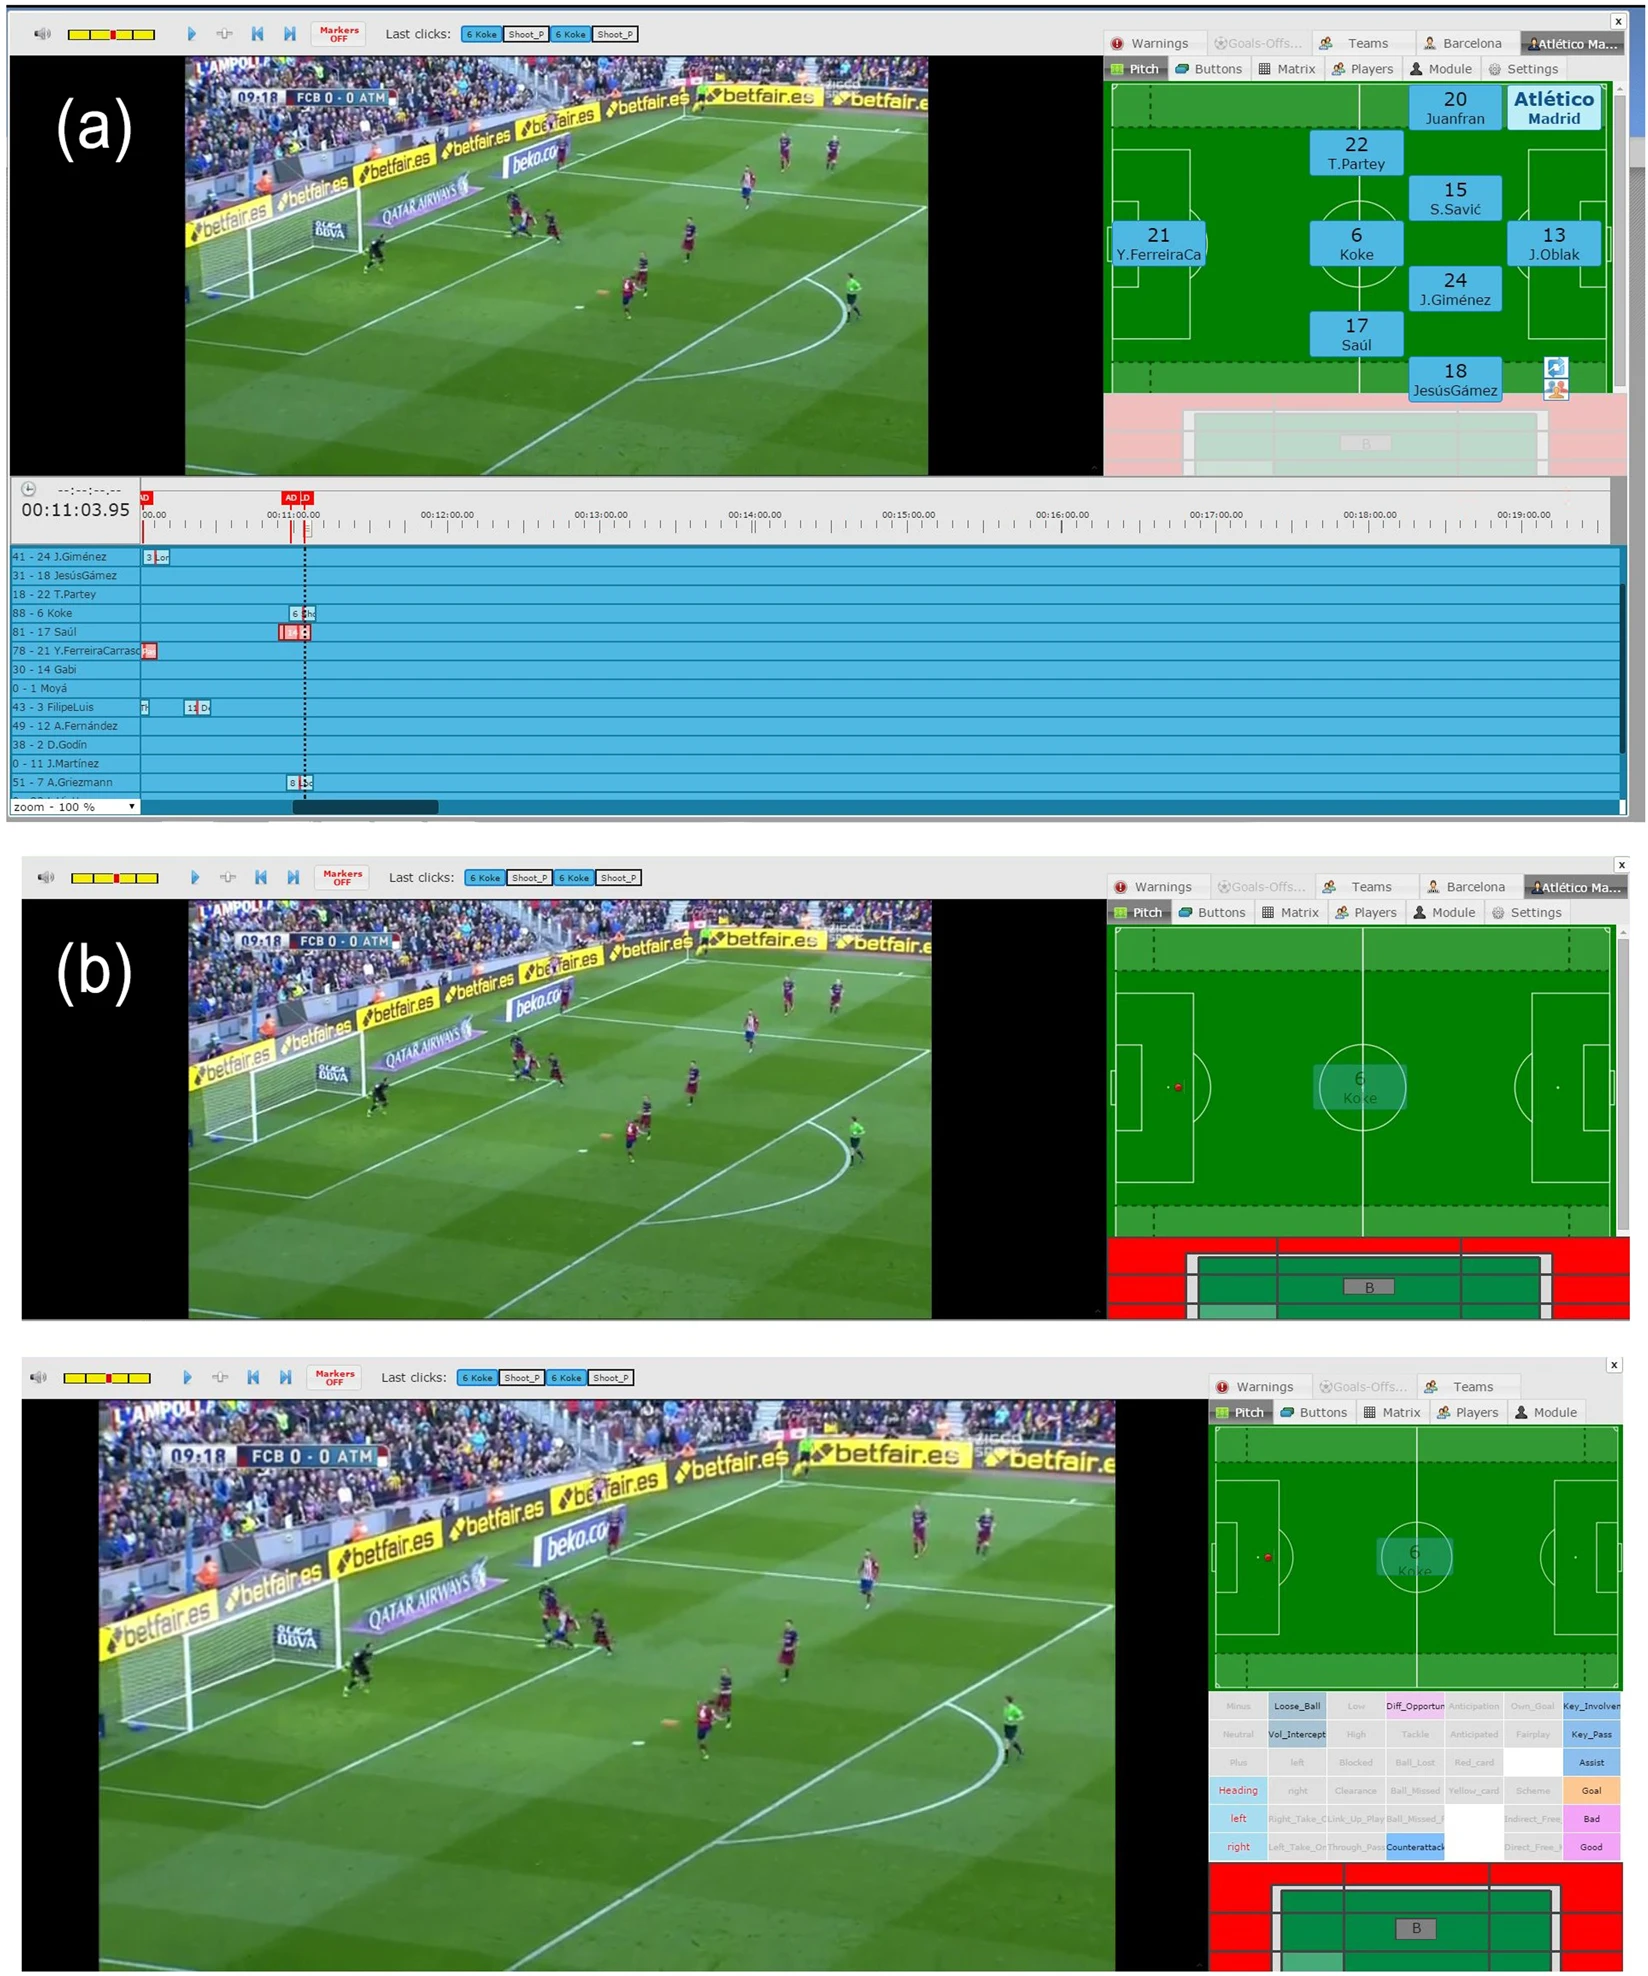
\includegraphics[width=0.7\textwidth]{img/logiciel_proprietaire.png}
    \caption{Aperçu du logiciel propriétaire de Wyscout}
    \label{fig:logiciel_proprietaire}
\end{figure}
\newline\newline
Le dataset utilisé est un sample du dataset de Wyscout. 
Il a été mis à disposition par Luca Pappalardo et Emanuele Massuco dans leur article "A public data set of spatio-temporal match events in soccer competitions" \cite{pappalardoPublicDataSet2019}.
\newline
Ce dataset est composé des 5 championnats européens majeurs (Premier League, La Liga, Bundesliga, Serie A et Ligue 1) de la saison 2017-2018. 
Le dataset contient également les informations de la Coupe du Monde 2018 et de l'Euro 2016.
Les données sont au format JSON qui est un format très récurrent dans le monde du web. Il est également utilisé lors de communication avec des API REST.

% Description de chaque attribut dans le dataset event
\subsection{Events}
\label{subsec:events}
% Utiliser le tableau de la thèse de Luca Pappalardo
% Egalement utiliser le glossaire de Wyscout pour expliquer les tag id
Le dataset fournit par Luca Pappalardo et Emanuele Massuco contient des données sur les événements d'un match. 
Ces événements sont décrits par des attributs qui sont détaillés dans le tableau \ref{tab:events}.
\begin{table}[htp]
    \centering
    \begin{tabular}{|l|l|}
    \hline
    \textbf{Nom de l'attribut} & \textbf{Description}                                                                                                                           \\ \hline
    eventId                    & \begin{tabular}[c]{@{}l@{}}L'identifiant du type d'événement. \\ Chaque identifiant d'événement \\ est lié à un nom d'événement\end{tabular}   \\ \hline
    eventName                  & Le nom du type d'événement.                                                                                                                    \\ \hline
    subEventId                 & L'identifiant du sous-type d'événement                                                                                                         \\ \hline
    subEventName               & Le nom du sous-événement                                                                                                                       \\ \hline
    tags                       & \begin{tabular}[c]{@{}l@{}}Une liste d'événement de tag.\\ Chaque tag permet d'apporter\\ une information\end{tabular}                         \\ \hline
    eventSec                   & \begin{tabular}[c]{@{}l@{}}Le temps (en secondes) écoulé depuis\\ la période actuelle du match\end{tabular}                                    \\ \hline
    id                         & L'identifiant unique de l'événement                                                                                                            \\ \hline
    matchId                    & \begin{tabular}[c]{@{}l@{}}L'identifiant du match auquel \\ l'événement est lié.\end{tabular}                                                  \\ \hline
    matchPeriod                & \begin{tabular}[c]{@{}l@{}}La période du match à laquelle \\ l'événement a lieu.\end{tabular}                                                  \\ \hline
    playerId                   & \begin{tabular}[c]{@{}l@{}}L'identifiant du joueur qui a généré\\ l'événement. Est lié à l'attribut "wyId"\\ du dataset "Players"\end{tabular} \\ \hline
    positions                  & La localisation en X et Y de l'événement                                                                                                       \\ \hline
    teamId                     & \begin{tabular}[c]{@{}l@{}}L'identifiant de l'équipe du joueur qui a \\ généré l'événement\end{tabular}                                        \\ \hline
    \end{tabular}
    \caption{Description des attributs du dataset "Events"}
    \label{tab:events}
\end{table}

Parmi les informations fournies par le dataset, il y a "eventName".
Cet attribut permet de savoir quel type d'événement a eu lieu.
Parmi les types d'événements\footnote{Le nom des événements est en anglais mais a été traduit pour les lister}, il y a :
\begin{itemize}
    \item Passe
    \item Faute
    \item Tir 
    \item Duel
    \item Coup franc
    \item Hors-jeu
    \item Touche de balle
\end{itemize}

L'attribut "tags" est également important.
Il représente une liste de tags qui permettent d'apporter des informations supplémentaires sur l'événement.
La documentation des tags peut être trouvée sur le glossaire de Wyscout. \cite{WyscoutGlossary}
Par exemple, le tag 101 indique que l'événement est un but. 
Le tag 401 indique que le tir a été fait du pied gauche, le tag 402 indique que le tir a été fait du pied droit.
Finalement, le tag 403 indique que le tir a été fait de la tête.
\newline\newline
Le dernier point important est la localisation de l'événement.
En effet, comme indiqué dans la section "Pitch coordinates" du glossaire de Wyscout, \cite{WyscoutGlossary} les coordonnées X et Y sont relatives à la taille du terrain.
Il y a un aperçu de la taille du terrain avec ses coordonnées sur la figure \ref{fig:terrain}.
Cela donne une idée de la taille du terrain.
Le choix de la taille du terrain en 100 par 100 a été fait car les terrains n'ont pas tous la même taille malgré les règles de l'IFAB.
\newline\newline
L'IFAB est l'International Football Association Board.
C'est un organisme qui définit les règles du football comme la taille des terrains.
Celle-ci pouvant varier entre 90 et 120 mètres de longueur et entre 45 et 90 mètres de largeur. \cite{TerrainIFAB}
\newline\newline 
Une autre information importante indiquée dans la documentation de l'API de Wyscout \cite{WyscoutAPI} est que les positions des événements ont été normalisées par rapport à l'emplacement du but de l'équipe qui a généré l'événement.
Cela veut dire que dans les données fournies par le dataset, les équipes jouent toujours dans le même sens du terrain.
Nous pouvons d'ailleurs constater cela lorsque nous regardons les positions des événements de tirs \ref{fig:events_tirs_emplacements}, en effet sur la figure \ref{fig:events_tirs_emplacements}, nous pouvons voir que les tirs sont toujours effectués du même côté du terrain\footnote{Certains sont effectuées dans l'autre partie du terrain mais jamais dans la surface de réparation opposée.}.
Il est également possible de visualiser la distribution des positions X des tirs sur la figure \ref{fig:histogramme_position_x_tirs}.
Nous pouvons apercevoir que les tirs sont toujours effectués dans la même partie du terrain.
Les tirs sont relatifs à la position du but de l'équipe qui a généré l'événement.
Cela règle déjà un problème qui aurait pu se poser.
En effet, il aurait fallu déterminer quelle équipe joue dans quel sens du terrain et donc savoir dans quelle direction les tirs sont effectués.
Ce travail aurait été nécessaire et extrêmement important car cela aurait pu fausser les données sur la distance et l'angle de tir.
\newline\newline
Nous savons donc que, dans le dataset, les équipes jouent toutes dans le même sens du terrain, Cela nous simplifie la tâche pour la suite de la thèse.

\begin{figure}[htp]
    \centering
    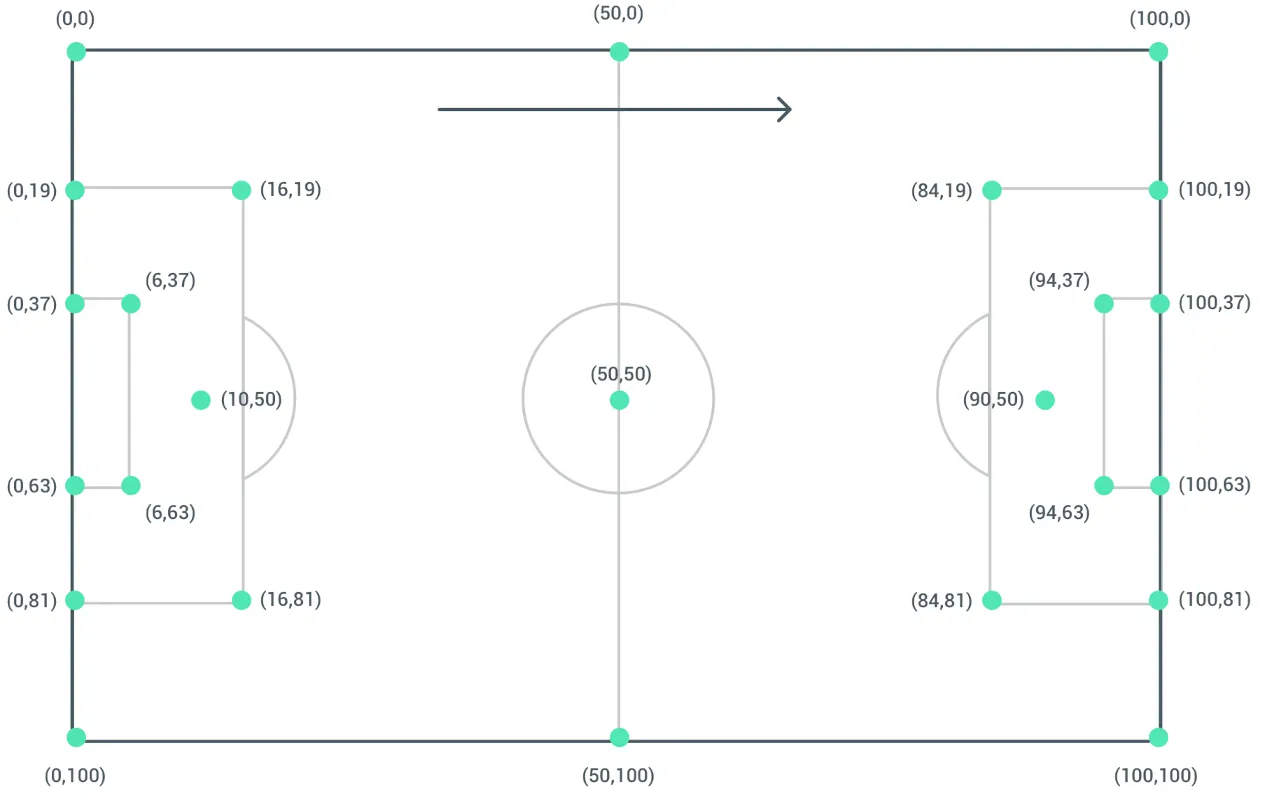
\includegraphics[width=0.8\textwidth]{img/CoordTerrain.png}
    \caption{Représentation du terrain de football avec les coordonnées X et Y}
    \label{fig:terrain}
\end{figure}

\begin{figure}[htp]
    \centering
    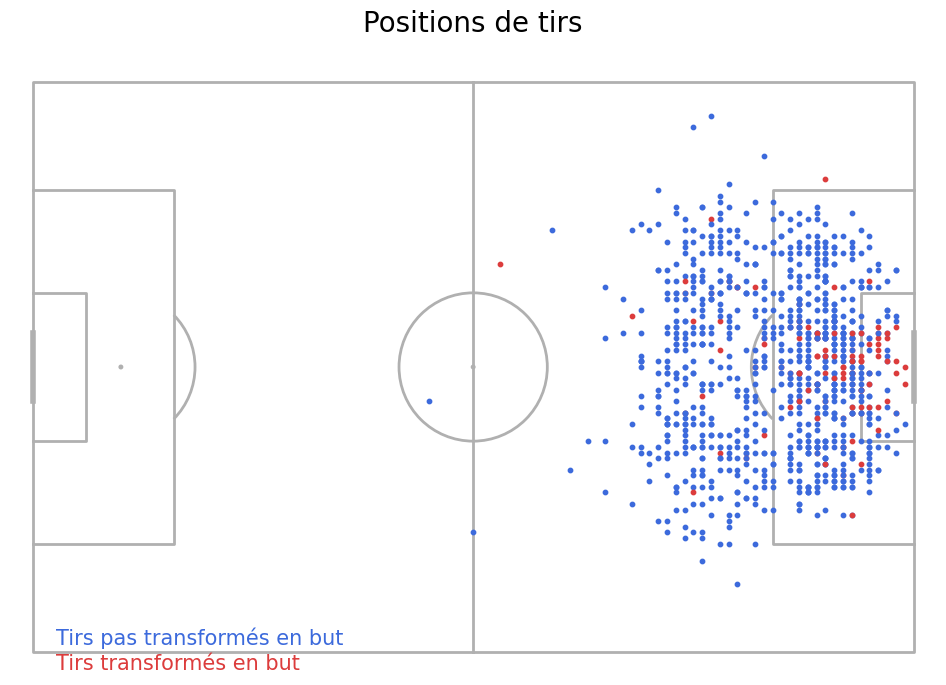
\includegraphics[width=0.8\textwidth]{img/PositionTirsDatasetEvent.png}
    \caption{Représentation des positions des 1000 premiers tirs}
    \label{fig:events_tirs_emplacements}
\end{figure}

\begin{figure}
    \centering
    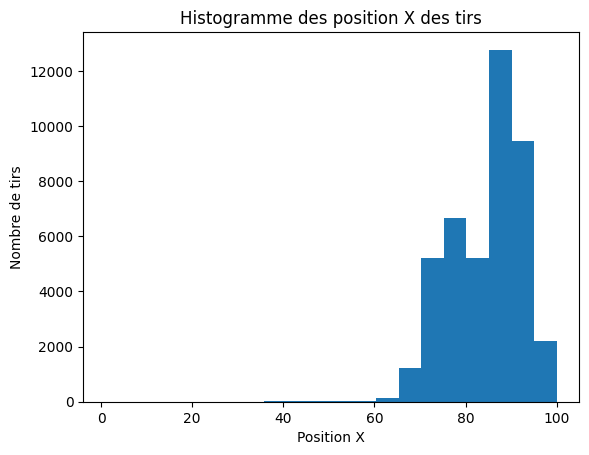
\includegraphics[width=0.8\textwidth]{img/histogramme_position_x_tirs.png}
    \caption{Histogramme des positions X des tirs}
    \label{fig:histogramme_position_x_tirs}
\end{figure}



\newpage
% Description de chaque attribut dans le dataset players
\subsection{Players}
Le dataset contient également des informations sur les joueurs.
Le tableau \ref{tab:players} décrit les attributs du dataset "Players".
\newline\newline
Nous pouvons voir que le dataset contient des informations sur les joueurs comme leur taille, leur poids, leur date de naissance, leur nationalité, leur poste, etc.
L'une des informations intéressante dans la suite de la thèse est le pied fort du joueur.
En effet, celui-ci peut être un facteur qui influence le résultat de la prédiction des xG.
C'est pour cela qu'il est important de garder cet attribut dans le dataset final qui sera utilisé pour entraîner le modèle.
\begin{table}[h]
    \centering
    \begin{tabular}{|l|l|}
    \hline
    \textbf{Nom de l'attribut} & \textbf{Description}                                                                                              \\ \hline
    birthArea                  & Pays de naissance du joueur                                                                                       \\ \hline
    birthDate                  & Date de naissance du joueur                                                                                       \\ \hline
    currentNationalTeamId      & Equipe nationale du joueur                                                                                        \\ \hline
    currentTeamId              & \begin{tabular}[c]{@{}l@{}}Equipe actuelle du joueur. \\ Est lié à l'attribut "wyId" de l'équipe\end{tabular}     \\ \hline
    firstName                  & Prénom du joueur                                                                                                  \\ \hline
    lastName                   & Nom du joueur                                                                                                     \\ \hline
    foot                       & Pied fort du joueur                                                                                               \\ \hline
    height                     & Taille du joueur en centimètres                                                                                   \\ \hline
    middleName                 & \begin{tabular}[c]{@{}l@{}}Deuxième nom du joueur. S'il en \\ possède un\end{tabular}                             \\ \hline
    passportArea               & Nationalité du joueur                                                                                             \\ \hline
    role                       & Poste du joueur                                                                                                   \\ \hline
    shortName                  & Nom raccourci du joueur                                                                                           \\ \hline
    weight                     & Poids du joueur en kilogrammes                                                                                    \\ \hline
    wyId                       & \begin{tabular}[c]{@{}l@{}}Identifiant du joueur.\\ Permet de faire le lien avec le dataset "Events"\end{tabular} \\ \hline
    \end{tabular}
    \caption{Description des attributs du dataset "Players"}
    \label{tab:players}
\end{table}

\newpage
\subsection{Transformation des données}
% Parler du présupposé de la taille du terrain 105x68
% Transformation des positions des événements en angle et distance
Comme discuté dans la section \ref{subsec:events}, les coordonnées X et Y sont relatives à la taille du terrain.
Un présupposé qui est fait est que la taille du terrain est de 105 par 68.
Celle-ci est la plus commune dans le football professionnel.
Nous pouvons notamment le voir sur le site officiel de la Premier League \cite{PremierLeagueClubs}.
Nous démarrons donc par un présupposé que tous les terrains qui ont accueilli les matchs dans le dataset ont comme dimension 105 mètres par 68.
Ce présupposé nous permettra ainsi de pouvoir calculer la distance en mètre par rapport au but adverse ainsi que l'angle de tir.
\newpage
Nous élaborerons notre travail sur la transformation des données en quatre parties distinctes.
Pour commencer, nous transformons les coordonnées X et Y qui sont à l'échelle 100 par 100 en coordonnées X et Y à l'échelle 105 par 68.
Pour cela, il suffit de multiplier les coordonnées X par 1.05 et les coordonnées Y par 0.68.
\begin{equation}
    \begin{split}
        x_{105} = x_{100} * 1.05 \\
        y_{68} = y_{100} * 0.68
    \end{split}
\end{equation}
Nous passons également les coordonnées X de l'autre côté du terrain. 
Cela permettra de calculer la distance par rapport au centre du terrain.
Il suffit de soustraire les coordonnées X à 105\footnote{Dans notre cas, nous soustrayons les coordonnées avant de passer à l'échelle 105x68, donc nous avons soustrait les coordonnées de X à 100.}.
\newline\newline
Par la suite, nous allons créer un attribut qui contient la distance par rapport au centre du terrain sur l'axe Y.
Cet attribut permettra de calculer la distance du tir ainsi que son angle.
Pour cela, il suffit de calculer la distance entre le centre du terrain et la position du tir, mais uniquement sur l'axe Y.
\begin{equation}
    \begin{split}
        y_{Centre} = \lvert y_{68} - 34 \rvert
    \end{split}
\end{equation}
34 étant la moitié de la largeur du terrain. 
Cela nous permet d'avoir la distance par rapport au centre du terrain sur l'axe Y \footnote{Tout comme pour la coordonnée X, la soustraction a été faite sur l'échelle 100x100 avant de passer à l'échelle 105x68}.
\newline\newline
Ensuite, nous calculons la distance du tir par rapport au but adverse.

Sur la figure \ref{fig:distance_tir}, [C] représente le centre du terrain, [E] représente le centre du but adverse.
[DG] représente l'attribut que l'on a calculer précédemment qui contient la distance par rapport au centre du terrain sur l'axe Y.
[DF] représente la position en X par rapport au but adverse.
Ce qui est effectué pour calculer la distance du tir par rapport au but adverse est d'utiliser le théorème de Pythagore.
Nous pouvons voir sur la figure \ref{fig:distance_tir} que nous avons un triangle rectangle [GDF].
Avec le théorème de Pythagore, nous pouvons savoir que :
\begin{equation}
    DE^2 = GF^2 = DG^2 + DF^2
\end{equation}
Il suffit de faire une racine carré de la somme de $DG^2$ et $DF^2$ pour avoir la distance du tir par rapport au centre du but adverse.
\newline\newline
Pour finir, nous allons calculer l'angle du tir par rapport au but adverse.
Il est d'abord important d'amener une autre information qui, cette fois-ci, n'est pas un présupposé.
En effet, la largeur des buts de football est de 7.32 mètres \cite{TerrainIFAB}.
Pour cette partie, le choix a été d'utiliser l'inverse de la tangente et la règle qui dit que la somme des angles d'un triangle est égale à 180 degrés.
Grâce à cela, nous pouvons calculer l'angle du tir par rapport au but adverse.
Nous pouvons voir sur la figure \ref{fig:angle_tir} que l'on a un triangle JGF.
L'objectif est de calculer l'angle situé au sommet G.
On sait que GI représente $y_{Centre}$ et que HF représente la valeur de $x$.
FJ représente la largeur du but qui est, comme indiqué précédemment, de 7.32 mètres.
Nous pouvons donc avoir la valeur de GH et GK en additionnant ou soustrayant la moitié de la largeur du but à $y_{Centre}$.
\begin{equation}
    \begin{split}
        GH = y_{Centre} - \frac{7.32}{2} \\
        GK = y_{Centre} + \frac{7.32}{2}
    \end{split}
\end{equation}
En utilisant la tangente inverse, il est possible de calculer l'angle GJK ainsi que l'angle GFH.
Avec ces deux angles, nous pouvons calculer l'angle à l'intérieur du triangle JGF pour finalement récupérer l'angle du tir par rapport au but adverse en faisant\footnote{En degrés} :
\begin{equation}
    \begin{split}
        \alpha = 180 - (Angle_{GJK} + Angle_{GFH})
    \end{split}
\end{equation}
Finalement l'équation totale ressemble à cela, une fois toutes les valeurs réunies :
\begin{equation}
    \begin{split}
        \alpha = 180 - (tan^{-1}(\frac{GH}{HF}) + 90) - (90 -tan^{-1}(\frac{GK}{HF}))
    \end{split}
\end{equation}

Il est d'ailleurs possible d'accéder aux schémas géométriques sur Geogebra.
Cela permet de manipuler les différents points et de voir les valeurs se mettre à jour automatiquement.
Ils sont disponibles en bas de page\footnote{Angle : \url{https://www.geogebra.org/geometry/d7tqw4fe}}\footnote{Distance : \url{https://www.geogebra.org/geometry/fnx3swex}}.

\begin{figure}[htp]
    \centering
    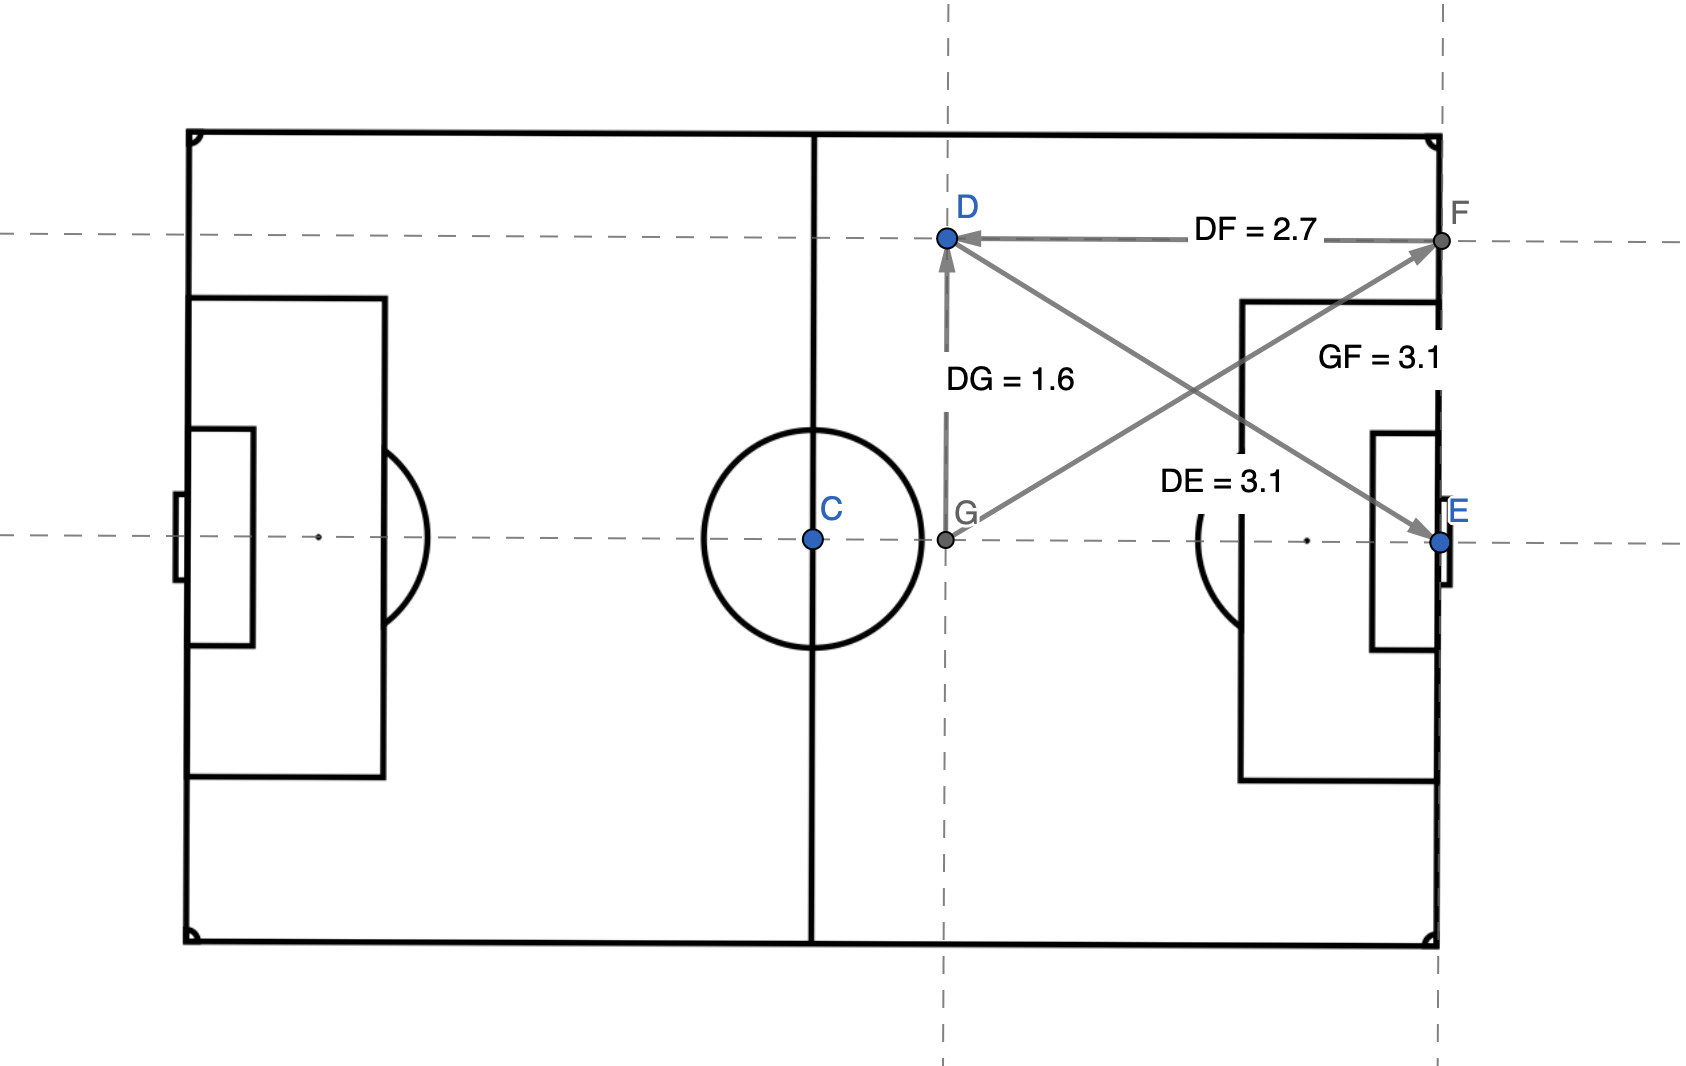
\includegraphics[width=0.9\textwidth]{img/schema_calcul_distance.png}
    \caption{Distance du tir par rapport au but adverse}
    \label{fig:distance_tir}
\end{figure}
\begin{figure}[htp]
    \centering
    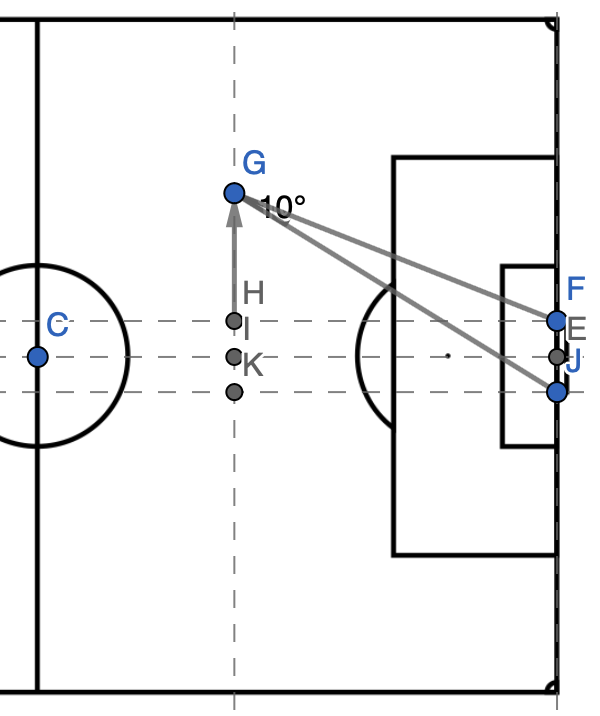
\includegraphics[width=0.5\textwidth]{img/schema_calcul_angle.png}
    \caption{Angle du tir par rapport au but adverse}
    \label{fig:angle_tir}
\end{figure}


\subsection{Fusion des datasets}
% Fusion des datasets events et players
Cette section vise à expliquer comment les datasets ont été fusionnés.
On a pu voir que le dataset events contient l'identifiant du joueur qui a effectué l'action sous le nom d'attribut "playerId" (voir table \ref{tab:events}).
Cet identifiant correspond à l'identifiant nommé "wyId" dans le dataset players (voir table \ref{tab:players}).
L'objectif est donc de fusionner les deux datasets en utilisant ces deux attributs pour permettre d'avoir les informations des joueurs dans le dataset events.
Dans notre cas, nous allons faire une jointure pour permettre d'identifier le pied fort du joueur ayant généré l'événement.
Grâce à cela, il nous est possible de savoir si le joueur a tiré avec son pied fort ou non.
\newline\newline

\begin{table}[htp]
    \centering
    \begin{tabular}{|l|l|}
        \hline
        \textbf{Nom de l'attribut} & \textbf{Description}                                                                                                                   \\ \hline
        X                          & \begin{tabular}[c]{@{}l@{}}Position X sur le terrain. Permet de visualiser les \\ tirs via un pitch chart\end{tabular}                 \\ \hline
        Y                          & \begin{tabular}[c]{@{}l@{}}Position Y sur le terrain. Permet de visualiser les \\ tirs via un pitch chart\end{tabular}                 \\ \hline
        distance                   & Distance du tir par rapport au milieu du but                                                                                           \\ \hline
        angle                      & \begin{tabular}[c]{@{}l@{}}Angle des deux poteaux par rapport au tir. En \\ radians\end{tabular}                                       \\ \hline
        angle\_abs                 & L'angle du tir par rapport au centre du terrain.                                                                                                      \\ \hline
        \textbf{goal}                       & Indique si le tir est un but. \textbf{La variable cible.}                                                                                                       \\ \hline
        header                     & \begin{tabular}[c]{@{}l@{}}Indique si le tir est fait de la tête. Si c'est le cas, \\ "good\_foot\_used" est False\end{tabular}        \\ \hline
        good\_foot\_used           & \begin{tabular}[c]{@{}l@{}}Indique si le tir est fait avec le pied fort du joueur.\\ Si c'est le cas, "header" est False.\end{tabular} \\ \hline
        \end{tabular}
    \caption{Attributs du dataset events}
    \label{tab:final_dataset}
\end{table}

\subsection{Visualisation des données}
% Visualisation des données
Cette section sert à visualiser les données du dataset final.
Tout d'abord, nous allons effectuer une description simple du dataset.
Le dataset contient 43075 tirs sur une saison de football (2017/2018) dans 7 compétitions différentes :
\begin{itemize}
    \item Ligue 1
    \item Premier League
    \item Serie A
    \item Bundesliga
    \item La Liga
    \item Coupe du monde 2018
    \item Euro 2016
\end{itemize}
La description du dataset est disponible sur le tableau \ref{tab:describe_dataset}.
Nous pouvons voir que la distance maximale d'un tir a été de 103.95 mètres et la distance minimale de 0.68 mètre.
Nous constatons que certains tirs n'ont pas été normalisés par rapport au sens du jeu de l'équipe comme indiqué dans la section \ref{subsec:events}. 
Notre but va être de retirer certains tirs considérés comme des "outliers".
\begin{table}[htp]
    \centering
    \begin{tabular}{r|r|r|r|r|r|}
        \cline{2-6}
        \textbf{}                   & \textbf{X}   & \textbf{Y}   & \textbf{distance} & \textbf{angle} & \textbf{angle\_abs} \\ \hline
        \multicolumn{1}{|r|}{count} & 43075 & 43075 & 43075      & 43075   & 43075        \\ \hline
        \multicolumn{1}{|r|}{mean}  & 15.99    & 33.47    & 18.59         & 0.4141       & 2.6576            \\ \hline
        \multicolumn{1}{|r|}{std}   & 8.53     & 9.37     & 8.42          & 0.2532       & 0.3131            \\ \hline
        \multicolumn{1}{|r|}{min}   & 0.00     & 0.00     & 0.68          & 0.0000       & 1.5708            \\ \hline
        \multicolumn{1}{|r|}{25\%}  & 9.45     & 26.52    & 12.25         & 0.25019       & 2.4418            \\ \hline
        \multicolumn{1}{|r|}{50\%}  & 13.65    & 33.32    & 17.15         & 0.3278       & 2.6894            \\ \hline
        \multicolumn{1}{|r|}{75\%}  & 23.10   & 40.80    & 24.94         & 0.5060       & 2.9143            \\ \hline
        \multicolumn{1}{|r|}{max}   & 103.95   & 68    & 103.95        & 3.1416       & 3.1416            \\ \hline
        \end{tabular}
    \caption{Description du dataset final}
    \label{tab:describe_dataset}
\end{table}

Tout d'abord, nous allons visualiser la fréquence des tirs en fonction de leur position à l'aide d'une heatmap sur un pitch chart.
Ce dernier est un graphique qui affiche un terrain de football.
Grâce à cela, nous pouvons apercevoir plus simplement d'où ont été effectués les tirs.
Le but de notre pitch chart est de visualiser les tirs qui ont été effectués à leurs positions respectives.
Dans notre cas, nous avons décidé d'utiliser une heatmap pour visualiser la fréquence des tirs à chacune des positions sur le terrain.
Le pitch chart peut être vu sur la figure \ref{fig:pitch_chart}.
Nous pouvons voir qu'une grande majorité des tirs ont été effectués dans la surface de réparation.
Nous sommes amenés à remarquer qu'il y a très peu de tirs à l'entrée de la surface de réparation.
Plusieurs hypothèses peuvent être faites pour expliquer cela.
La première est que les joueurs préfèrent tirer dans la surface de réparation car ils ont plus de chances de marquer. 
Cependant, nous remarquons qu'il y a également des tirs plus lointains.
La deuxième hypothèse est que ce phénomène est dû à comment les données sont récoltées.
Il est effectivement possible que les opérateurs ou que le logiciel propriétaire de Wyscout détermine qu'un tir ait été fait dans la surface de réparation ou en dehors de celle-ci, plutôt que sur la ligne de la surface de réparation.
Cela nous montre déjà une des limitations des données que nous utilisons.
\begin{figure}[htp]
    \centering
    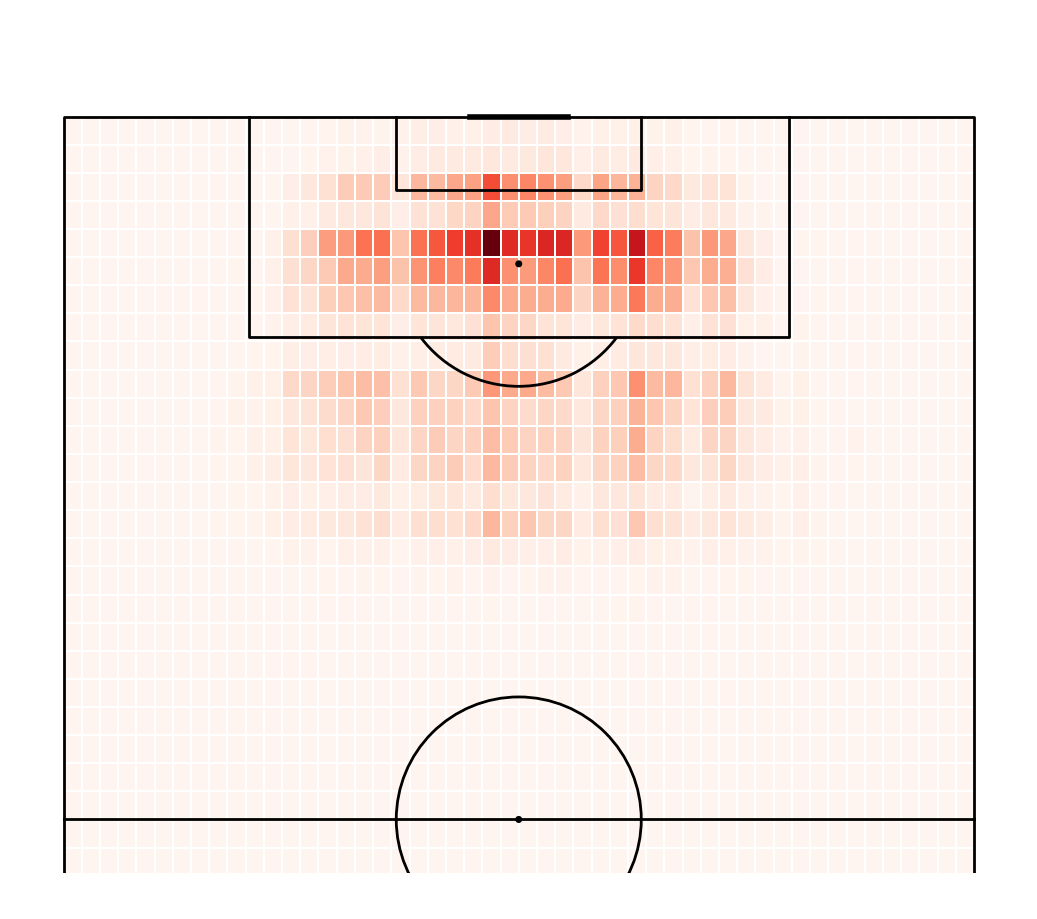
\includegraphics[width=0.8\textwidth]{img/pitchChartFrequency.png}
    \caption{Pitch chart des tirs effectués}
    \label{fig:pitch_chart}
\end{figure}

Maintenant, nous allons nous focaliser sur la détection d'éventuelles "outliers".
En effet, nous avons pu voir que la distance maximale d'un tir a été de 103.95 mètres. 
Il faut donc vérifier si ce tir est un "outlier" ou non. 
Nous allons également nous focaliser sur d'autres tirs considérés comme "outliers".
Tout d'abord, visualisons les graphiques de la distance, l'angle de tir et l'angle de tir absolu (voir fig. \ref{fig:analyse_quantitative}).
Lorsque nous observons les histogrammes, nous nous apercevons que pour la distance et l'angle de tir, il y a une majorité de tirs qui ont été effectués à une distance inférieure à 50 mètres et un angle de tir inférieur à 1.5 radian.
Nous pouvons également voir qu'il n'y a pas de séparation distincte entre les distributions des tirs selon leur valeur cible via les graphiques de la deuxième colonne.
Cela aurait été très pertinent puisque nous aurions pu voir quel attribut aurait été le plus influent directement en observant les données.
Cependant, nous pouvons remarquer que des outliers ont été trouvés pour la distribution des différentes variables via les boxplots. 
Les outliers sont déterminés en se basant sur la règle suivante \cite{galarnykUnderstandingBoxplotsHow2022} :
\begin{equation}
    \begin{split}
        x < Q_1 - 1.5 * IQR \\
        x > Q_3 + 1.5 * IQR    
    \end{split}
\end{equation}
Comme indiqué sur la documentation de Matplotlib concernant les boxplots \cite{MatplotlibPyplotBoxplot}, la valeur de 1.5 est une valeur basée sur la définition initiale des boxplots de John Tukey.
Ils permettent de définir les "maximum non-outlier" et "minimum non-outlier".
\newline
Via cette formule, nous sommes capables de récupérer tous les outliers pour chaque variable, nous obtenons un tableau comme celui-ci (voir tab. \ref{tab:outliers}):
L'objectif est maintenant de visualiser la probabilité de chacun des sets d'outliers. 
Si nous observons des anomalies ou des données aberrantes, il sera nécessaire de les supprimer.
\begin{table}[htp]
    \centering
    \begin{tabular}{l|l|l|l|}
        \cline{2-4}
        \multicolumn{1}{r|}{}                                                             & \textbf{Distance} & \textbf{Angle} & \textbf{Angle absolu} \\ \hline
        \multicolumn{1}{|l|}{\begin{tabular}[c]{@{}l@{}}Nombre\\ d'outliers\end{tabular}} & 197               & 2163           & 70                    \\ \hline
    \end{tabular}
    \caption{Outliers pour chaque variable quantitatives}
    \label{tab:outliers}
\end{table}

Grâce à la figure \ref{fig:analyse_outlier2}, plusieurs observations peuvent être faites. 
Tout d'abord, il est remarquable que les outliers pour les angles ne sont pas aberrants. 
En effet, théoriquement, plus l'angle est grand, plus le but est facile à réaliser. 
Cependant, en ce qui concerne les distances, il existe un nombre très limité d'outliers. 
En examinant les valeurs situées entre 90 et 105, nous pouvons constater que trois buts ont été marqués à cette distance. 
En revanche, le nombre de tirs manqués dans la même plage est plus élevé.
Théoriquement, marquer un but à 90 mètres du but est considéré comme irréalisable. 
Par conséquent, ces données peuvent être considérées comme aberrantes et il serait envisageable de les supprimer. 
Une hypothèse plausible est que ces données n'ont pas été correctement traitées par Wyscout lors de la normalisation des positions des tirs.
\newline\newline
Il est également intéressant d'examiner la relation entre la distance et l'angle. 
La figure \ref{fig:analyse_qualitative} met en évidence le fait que plus la distance est petite, plus l'angle est grand. 
Cette tendance est observée dans le premier graphique de la figure \ref{fig:analyse_qualitative}, bien que ce ne soit pas toujours le cas. 
En jouant avec le graphique Geogebra fourni précédemment, il est possible de constater que les tirs effectués depuis le coin de l'équipe attaquante auront un angle plus élevé que les tirs effectués depuis le coin de l'équipe adverse.
Un tir depuis le corner de l'équipe adverse aura systématiquement un angle de 0 radian puisqu'il est effectué le long de la ligne de but.
\newline\newline
Ensuite, nous allons analyser les attributs qualitatifs en utilisant des diagrammes en barres (bar charts). 
Ces graphiques permettent de visualiser la distribution des données pour chaque attribut qualitatif. 
Ils sont présentés dans la figure \ref{fig:analyse_qualitative}. 
À travers ces bar charts, il est possible d'observer que 10\% des tirs sont des buts. 
Nous constatons également qu'il y a une majorité de tirs effectués avec le pied fort du tireur. 
Cependant, les tirs qui ne sont pas effectués avec le pied fort incluent également les tirs de la tête.
Environ 15\% des tirs sont réalisés de cette manière, ce qui indique que la majorité des tirs sont effectués avec le pied (faible ou fort).
\newline\newline
Enfin, nous allons analyser la corrélation entre les variables.
L'objectif de cette analyse est d'évaluer si les variables sont corrélées les unes avec les autres.
Pour rappel, deux variables sont corrélées si elles ont tendance à varier ensemble. 
Une corrélation négative indique que lorsque la valeur d'une variable augmente, la valeur de l'autre variable diminue. 
Une corrélation positive indique que la valeur d'une variable augmente lorsque la variable corrélée augmente également.
Une corrélation élevée suggère une relation claire entre une variable et la variable cible, ce qui peut faciliter la compréhension de l'influence entre les deux variables.
Une corrélation élevée peut améliorer la prédiction et faciliter l'interprétation du modèle. 
\newline\newline
Dans notre cas, en observant la figure \ref{fig:correlation_matrix}, les variables présentant la corrélation la plus élevée par rapport à l'attribut "goal" sont les attributs "distance" et "angle". 
Nous remarquons également une forte corrélation entre les attributs "distance" et "X". 
Cette corrélation s'explique par le fait que l'attribut "distance" est une variable dérivée de l'attribut "X" et de l'attribut "C" qui est elle-même dérivée de l'attribut "Y".
\begin{figure}[htp]
    \centering
    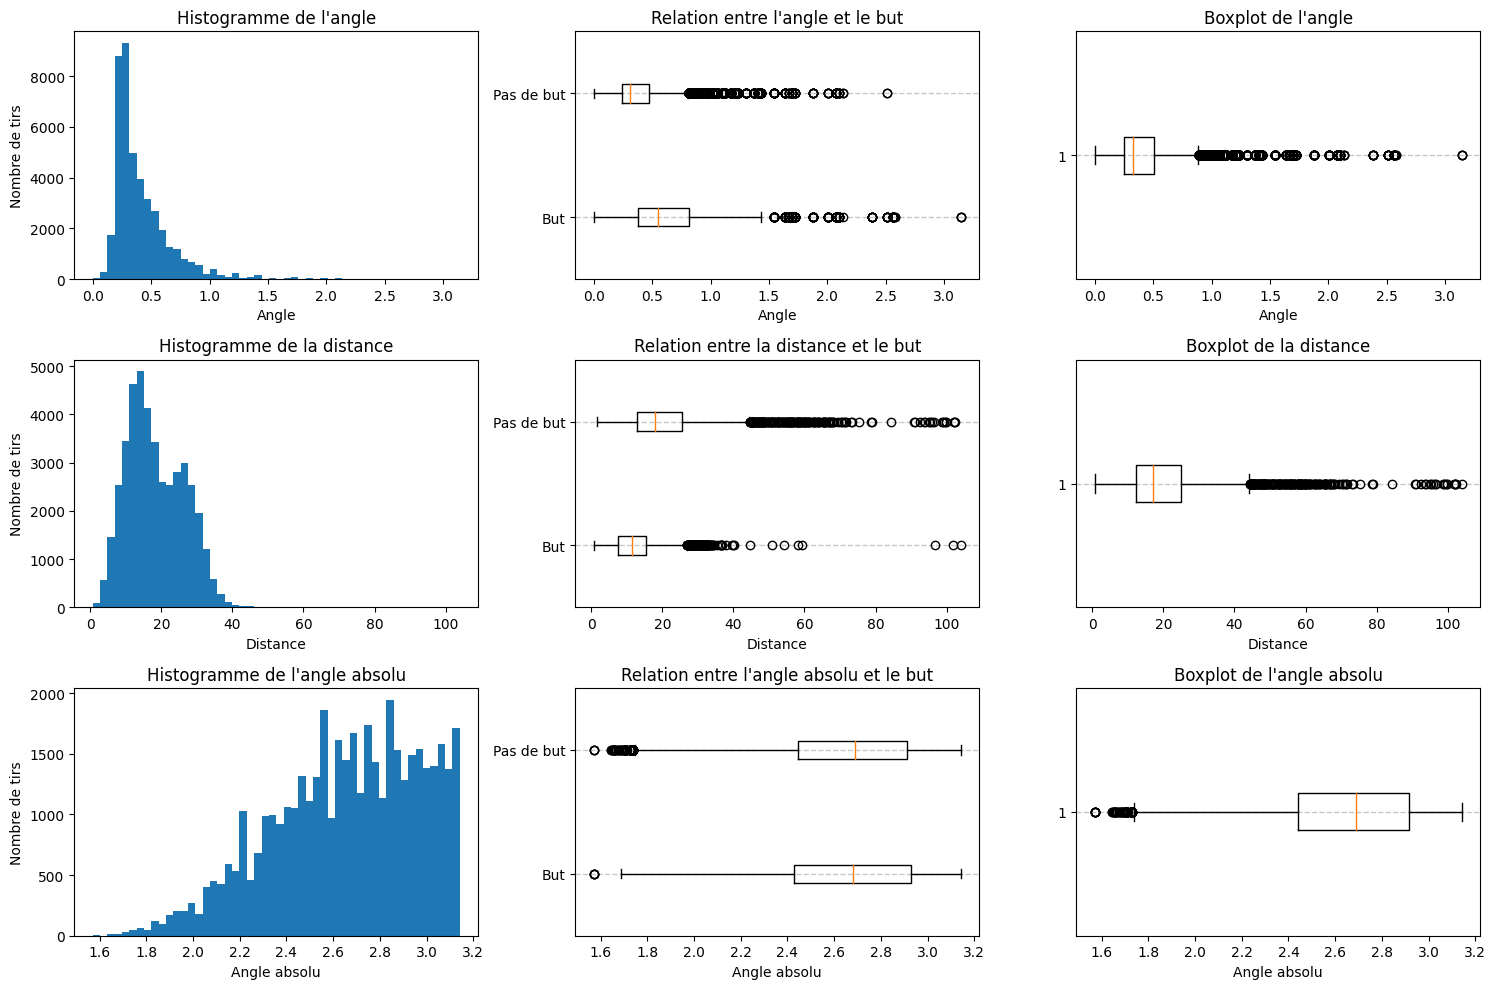
\includegraphics[width=\textwidth]{img/analyseOutlier.png}
    \caption{Analyse des attributs quantitatifs}
    \label{fig:analyse_quantitative}
\end{figure}

\begin{figure}[htp]
    \centering
    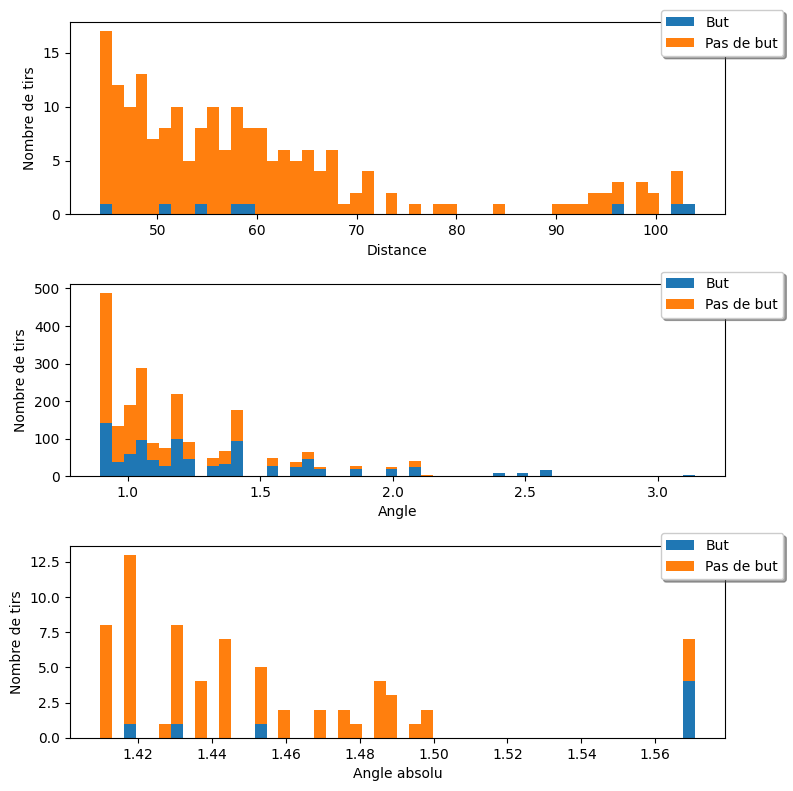
\includegraphics[width=\textwidth]{img/analyseOutlier2.png}
    \caption{Analyse des outliers}
    \label{fig:analyse_outlier2}
\end{figure}
\begin{figure}[htp]
    \centering
    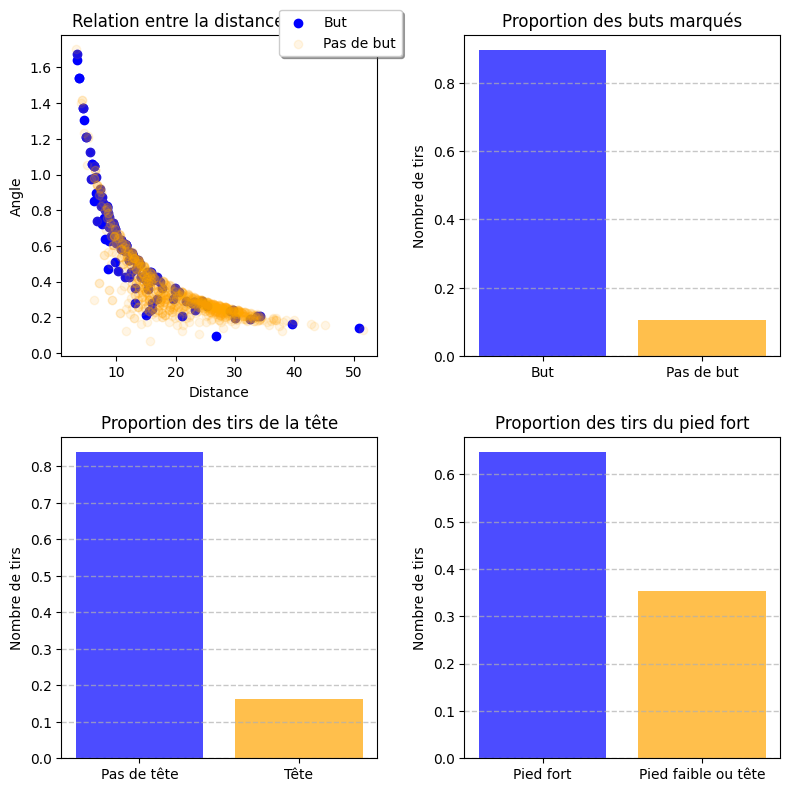
\includegraphics[width=\textwidth]{img/visualisation_discret.png}
    \caption{Relation distance-angle et analyse des attributs qualitatifs}
    \label{fig:analyse_qualitative}
\end{figure}

\begin{figure}
    \centering
    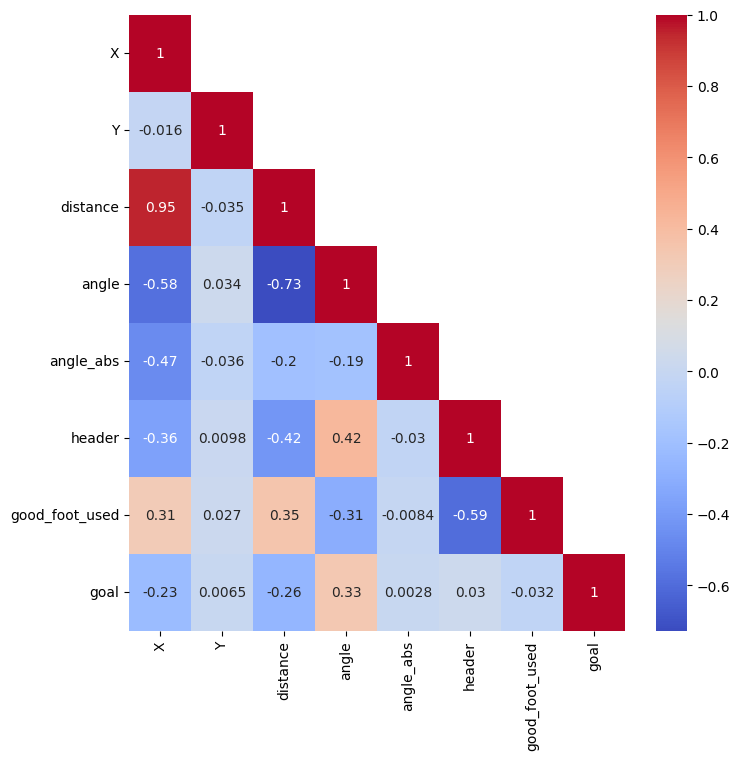
\includegraphics[width=\textwidth]{img/correlation_matrix.png}
    \caption{Matrice de corrélation des attributs}
    \label{fig:correlation_matrix}
\end{figure}
\newpage
Grâce à cette visualisation approfondie, nous avons pu acquérir une compréhension approfondie des données et des relations entre les différentes variables. 
Nous avons également identifié certaines données incohérentes et des aberrations dans le jeu de données. 
Ces observations soulignent l'importance de l'examen attentif et critique des données afin d'éliminer les valeurs aberrantes et d'obtenir des résultats plus fiables.
\newline\newline
En analysant les corrélations entre les variables, nous avons constaté que certaines d'entre elles présentaient une forte corrélation avec la variable cible. 
Cela suggère que ces variables sont des indicateurs significatifs pour prédire la réussite d'un tir au but. 
Par exemple, les variables "distance" et "angle" ont montré une corrélation élevée avec la variable "goal". 
Cela signifie que plus la distance et l'angle sont favorables, plus la probabilité de marquer un but est élevée. 
\newline\newline
Il est essentiel de noter que la variable "distance" présente une corrélation significative avec la variable "X". 
Cette corrélation découle du fait que le calcul de l'attribut "distance" repose sur les coordonnées horizontales "X" et "C". 
Par conséquent, toute modification de la valeur de l'attribut "X" a un impact direct sur la valeur de l'attribut "distance".
\newline\newline
En résumé, cette analyse approfondie des données nous a permis de mieux comprendre les relations entre les variables et d'identifier les facteurs les plus pertinents pour prédire la réussite d'un tir au but. 
En éliminant les données aberrantes et en tenant compte des corrélations significatives, nous pouvons améliorer la précision des prédictions.
Cependant, il convient de noter que des analyses supplémentaires et des modélisations plus avancées peuvent être nécessaires pour tirer des conclusions plus précises et éclairantes.

\newpage
% Affichage de la visualisation suite au retour de Nils

\section{Méthodologie}
\label{sec:methodologie}
% Liste des méthodes qui vont être utilisées
Dans cette section, nous allons discuter de la méthodologie utilisée pour résoudre le problème de prédiction de la réussite d'un tir au but.
Tout d'abord, nous allons faire une séparation sur le dataset pour avoir un jeu de données d'entraînement et un jeu de données de test.
Le jeu de test sera utilisé pour évaluer la performance des modèles finaux. 
Tandis que le jeu d'entraînement, nous permettra d'entraîner notre modèle et de choisir le meilleur set d'hyper paramètres pour chaque modèle.
Le partitionnement choisi pour les jeux de données est le suivant : 90\% des données pour le jeu d'entraînement et 10\% des données pour le jeu de test.
Ayant environ 43'000 tirs enregistrés, cela nous donne approximativement 38'700 tirs pour le jeu d'entraînement et 4'300 tirs pour le jeu de test.
Ainsi, nous avons un jeu de données d'entraînement suffisamment vaste pour entraîner nos modèles et un jeu de test de taille adéquate pour évaluer leur performance.

\subsection{Choix des modèles}
Plusieurs modèles vont être utlisés pour résoudre ce problème.
Nous allons utiliser des modèles de classification binaire, car nous cherchons à prédire si un tir au but est réussi ou non.
Il est important de rappeler que le but de la thèse est de répondre à la question suivante : "Quels sont les paramètres qui influencent le plus l'expected goal ?".
Certains de ces modèles ne seront pas les plus performants et les plus cohérents pour avoir la meilleure prédiction possible mais ils permettront de comprendre les paramètres qui influencent le plus l'expected goal.
Nous allons tester les modèles suivants :
\begin{itemize}
    \item Régression logistique
    \item Arbre de décision
    \item Random Forest
    \item KNN
    \item Réseau de neurones (MLP)
\end{itemize}
Le choix de ces modèles est basé sur les modèles les plus utilisés pour des problèmes de classification.
Nous avons choisi ces modèles car ils sont tous différents et permettent de tester différentes approches pour résoudre le problème.
De plus, pour des questions de puissance de calcul, nous avons choisi des modèles qui ne sont pas trop complexes permettant d'être exécutés sur un ordinateur personnel.


\subsection{Cross Validation}
\label{sec:cross_validation}
Pour chaque modèle, nous allons utiliser la cross validation pour choisir le meilleur set d'hyper paramètres.
Elle représente une méthode qui permet de tester la performance d'un modèle sur un jeu de données.
Elle consiste à séparer le jeu de données en plusieurs sous-ensembles.
Comme nous pouvons le voir sur la figure \ref{fig:cross_validation}, le jeu de données est séparé en 5 sous-ensembles.
Chaque itération consiste à entraîner le modèle sur 4 sous-ensembles et à tester le modèle sur le dernier sous-ensemble (celui de "Validation").
Cette opération est répétée 5 fois pour que chaque sous-ensemble soit utilisé comme jeu de test.
La performance du modèle est calculée en faisant la moyenne des performances obtenues sur chaque sous-ensemble.
Dans notre cas, cette performance est effectuée en utilisant la "log loss" comme métrique.
Celle-ci est utilisée dans des contextes de classification probabiliste\footnote{Pour rappel, le xG est une métrique probabiliste puisqu'elle indique la chance qu'un tir soit transformé en but sous forme de pourcentage.} permettant d'évaluer la performance d'un modèle de classification.
Ainsi, nous pouvons choisir le meilleur set d'hyper paramètres pour chaque modèle.
\newline\newline
Après avoir choisi nos modèles et leurs hyper paramètres, nous allons les entraîner sur le jeu de données d'entraînement entier et les tester sur le jeu de données de test final.
Cela nous permettra ensuite de comparer les résultats entre les différents modèles.
Le but est d'avoir la meilleure version d'un modèle et de la comparer avec la meilleure version des autres modèles. 
C'est ainsi que nous pourrons déterminer quel modèle est le plus performant pour résoudre notre problème.
\begin{figure}[htp]
    \centering
    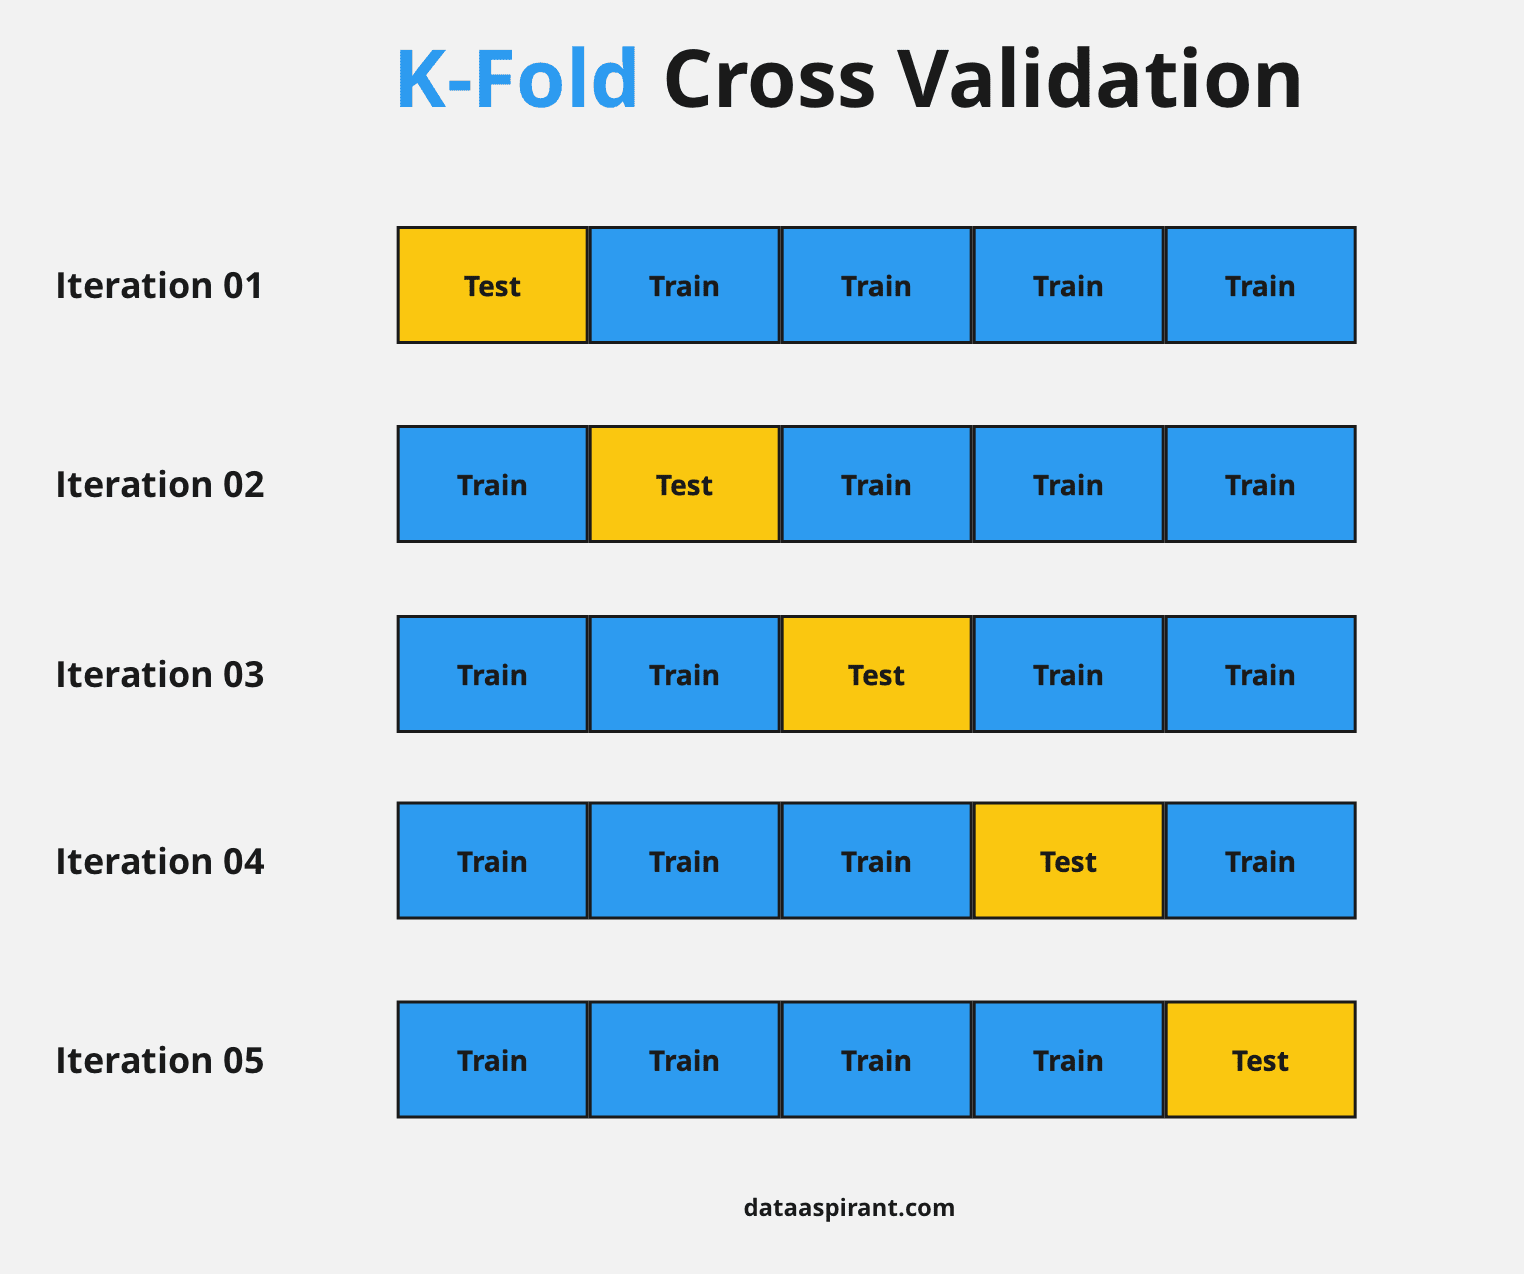
\includegraphics[width=0.7\textwidth]{img/cross_validation_schema.png}
    \caption{Cross Validation avec 5 sous-ensembles}
    \label{fig:cross_validation}
\end{figure}
\newpage
\subsection{Sélection des meilleurs attributs}
\label{sec:selection_attributs}
Pour la sélection des meilleurs attributs, nous allons utiliser la méthode de forward elimination.
Elle consiste à tester tous les attributs un par un en les ajoutant au fur et à mesure au modèle et observer la performance du modèle.
La p-value est utilisée pour déterminer si un attribut est significatif ou non et s'il apporte une amélioration à la performance du modèle.
Plus la p-value est faible, plus l'attribut est significatif.
\newline\newline
Par exemple, dans le tableau \ref{tab:logistic_regression_result_1}, nous sommes amenés à voir que l'attribut "X" a une p-value de 0.000.
Cela indique que cet attribut est significatif et qu'il apporte une amélioration à la performance du modèle en plus de la constante.
\newline\newline
Sur le tableau \ref{tab:logistic_regression_result_2}, nous pouvons voir que l'attribut "Y" a une p-value de 0.960.
Cela indique que cet attribut n'est pas du tout significatif et qu'il n'apporte aucune amélioration à la performance du modèle.
Nous pouvons le remarquer d'ailleurs lorsque nous observons la valeur du coefficient qui est très proche de 0.
Il faut donc supprimer cet attribut du modèle.
\newline\newline
Pour la troisième itération sur le tableau \ref{tab:logistic_regression_result_3}, nous ajoutons l'attribut "distance" au modèle.
Cependant, nous avons supprimé l'attribut "Y" qui n'était pas significatif.
Nous constatons que les p-values des attributs "X" et "distance" sont très faibles.
Cela indique que ces deux attributs sont significatifs et qu'ils apportent une amélioration à la performance du modèle.
La valeur du coefficient de l'attribut "distance" est négative. 
Cela veut dire que plus la distance est grande, plus la probabilité d'avoir un but est faible.
\newline\newline
Pour la quatrième itération sur le tableau \ref{tab:logistic_regression_result_4}, nous ajoutons l'attribut "angle" au modèle.
Cependant, dans ce cas-ci, nous observons que la p-value de l'attribut "X" est très élevée. 
Cela est dû à la corrélation entre les attributs "X" et "angle" qui est répétitive dû à leur lien avec l'attribut "distance".
C'est pour cela que l'attribut "X" n'est plus significatif et qu'il n'apporte plus d'amélioration à la performance du modèle.
Cela est dû au fait que l'attribut "distance" et l'attribut "angle" sont des attributs dérivés de l'attribut "X" et de l'attribut "Y".
\newline\newline
Lors de la cinquième itération, nous ajoutons l'attribut "angle\_abs" au modèle.
Ici, nous pouvons apercevoir que la p-value de l'attribut "angle\_abs" est très élevée.
Cela est dû à la corrélation entre les attributs "angle" et "angle\_abs" qui est répétitive.
C'est pour cela que l'attribut "angle\_abs" n'est pas significatif et qu'il doit être retiré.
\newline\newline
Pour finir, nous pouvons voir sur le tableau \ref{tab:logistic_regression_result_6} que l'ajout de l'attribut "header" et "good\_foot\_used" apporte une amélioration significative au modèle.
Cela se voit grâce aux p-values très faibles de ces deux attributs lorsque nous les additionnons aux autres attributs du modèle.

\newpage
\begin{table}[htp]
    \centering
    \begin{tabular}{lllllll}
        \multicolumn{7}{c}{\textbf{Logistic Regression Result}}                        \\ \hline
              & coef    & std err & z       & P\textgreater{}|z| & {[}0.025 & 0.975{]} \\ \hline
        const & -0.4809 & 0.037   & -13.120 & 0.000              & -0.553   & -0.409   \\
        X     & -0.1280 & 0.003   & -42.743 & 0.000              & -0.134   & -0.122   \\ \hline
        \end{tabular}
    \caption{Résultats de la régression logistique - 1ère itération}
    \label{tab:logistic_regression_result_1}
\end{table}
\begin{table}[htp]
    \centering
    \begin{tabular}{lllllll}
    \multicolumn{7}{c}{\textbf{Logistic Regression Result}}                          \\ \hline
          & coef      & std err & z       & P\textgreater{}|z| & {[}0.025 & 0.975{]} \\ \hline
    const & -0.4843   & 0.076   & -6.334  & 0.000              & -0.634   & -0.334   \\
    X     & -0.1280   & 0.003   & -42.729 & 0.000              & -0.134   & -0.122   \\
    Y     & 9.939e-05 & 0.002   & 0.050   & 0.960              & -0.004   & 0.004   \\ \hline
    \end{tabular}
    \caption{Résultats de la régression logistique - 2ème itération}
    \label{tab:logistic_regression_result_2}
\end{table}
\begin{table}[htp]
    \centering
    \begin{tabular}{lllllll}
    \multicolumn{7}{c}{\textbf{Logistic Regression Result}}                           \\ \hline
             & coef    & std err & z       & P\textgreater{}|z| & {[}0.025 & 0.975{]} \\ \hline
    const    & 0.1926  & 0.043   & 4.488   & 0.000              & 0.108    & 0.277    \\
    X        & 0.0692  & 0.008   & 8.579   & 0.000              & 0.053    & 0.085    \\
    distance & -0.2118 & 0.008   & -26.825 & 0.000              & -0.227   & -0.196   \\ \hline
    \end{tabular}
    \caption{Résultats de la régression logistique - 3ème itération}
    \label{tab:logistic_regression_result_3}
\end{table}

\begin{table}[htp]
    \centering
    \begin{tabular}{lllllll}
    \multicolumn{7}{c}{\textbf{Logistic Regression Result}}                           \\ \hline
             & coef    & std err & z       & P\textgreater{}|z| & {[}0.025 & 0.975{]} \\ \hline
    const    & -1.3884 & 0.123   & -11.294 & 0.000              & -1.629   & -1.147   \\
    X        & 0.0060  & 0.009   & 0.660   & 0.509              & -0.012   & 0.024    \\
    distance & -0.0984 & 0.011   & -8.799  & 0.000              & -0.120   & -0.076   \\
    angle    & 1.3701  & 0.102   & 13.395  & 0.000              & 1.170    & 1.571    \\ \hline
    \end{tabular}
    \caption{Résultats de la régression logistique - 4ème itération}
    \label{tab:logistic_regression_result_4}
\end{table}

\begin{table}[htp]
    \centering
    \begin{tabular}{lllllll}
    \multicolumn{7}{c}{\textbf{Logistic Regression Result}}                             \\ \hline
               & coef    & std err & z       & P\textgreater{}|z| & {[}0.025 & 0.975{]} \\ \hline
    const      & -1.3245 & 0.154   & -8.573  & 0.000              & -1.627   & -1.022   \\
    distance   & -0.0897 & 0.005   & -18.200 & 0.000              & -0.099   & -0.080   \\
    angle      & 1.4499  & 0.102   & 14.243  & 0.000              & 1.250    & 1.649    \\
    angle\_abs & -0.0592 & 0.064   & -0.932  & 0.352              & -0.184   & 0.065    \\ \hline
    \end{tabular}
    \caption{Résultats de la régression logistique - 5ème itération}
    \label{tab:logistic_regression_result_5}
\end{table}

\begin{table}[htp]
    \centering
    \begin{tabular}{lllllll}
    \multicolumn{7}{c}{\textbf{Logistic Regression Result}}                                   \\ \hline
                     & coef    & std err & z       & P\textgreater{}|z| & {[}0.025 & 0.975{]} \\ \hline
    const            & -1.0751 & 0.114   & -9.413  & 0.000              & -1.299   & -0.851   \\
    distance         & -0.1126 & 0.005   & -23.827 & 0.000              & -0.122   & -0.103   \\
    angle            & 1.5497  & 0.093   & 16.609  & 0.000              & 1.367    & 1.733    \\
    header           & -0.9067 & 0.059   & -15.468 & 0.000              & -1.022   & -0.792   \\
    good\_foot\_used & 0.1224  & 0.046   & 2.634   & 0.008              & 0.031    & 0.214    \\ \hline
    \end{tabular}
    \caption{Résultats de la régression logistique - Dernière itération}
    \label{tab:logistic_regression_result_6}
\end{table}
\newpage
Pour conclure cette partie de sélection d'attributs, nous constatons que les attributs les plus significatifs parmi ceux que nous avons sélectionné pour le dataset final sont :
\begin{itemize}
    \item La distance entre la position du tir et le but
    \item L'angle entre les deux poteaux et la position du tir
    \item Le tir a été effectué avec le pied fort du joueur
    \item Le tir a été fait de la tête
\end{itemize}
Nous pouvons donc en conclure que les attributs que nous avons sélectionné sont pertinents pour la prédiction de la réussite d'un tir. 
Il est également possible de voir que les attributs que nous avons sélectionné sont cohérents avec les résultats de la littérature. 
En effet, nous retrouvons les attributs suivants :
\begin{itemize}
    \item La distance entre la position du tir et le but
    \item L'angle entre les deux poteaux et la position du tir
\end{itemize}

Avec cette conclusion, nous avons pu répondre à la première question de la thèse : \newline\textbf{Quels sont les paramètres qui influencent le plus l’expected goal ?}


\subsection{Jeu d'hyper paramètres et séléction}
Pour le choix des hyper paramètres pour chacun des nos modèles, le but est d'utiliser une méthode de validation croisée.
Chacun des modèles sera créé avec un jeu d'hyper paramètres différent et passera par une validation croisée.
Chaque résultat de validation croisée sera ensuite comparé pour trouver le meilleur jeu d'hyper paramètres pour chaque modèle.
Comme indiqué dans la partie \ref{sec:cross_validation}, nous utiliserons une validation croisée à 5 folds pour chacun des modèles en utilisant la métrique du log loss.
Nous mettrons la méthode en grille pour trouver les meilleurs hyper paramètres pour chacun des modèles.
Il est possible de trouver les hyper paramètres les plus optimaux pour chacun des modèles relatifs à notre cas dans les tableaux \ref{tab:logistic_regression_hyperparameters}, \ref{tab:decision_tree_hyperparameters}, \ref{tab:random_forest_hyperparameters}, \ref{tab:knn_hyperparameters} et \ref{tab:mlp_hyperparameters} .
\begin{table}[htp]
    \centering
    \begin{tabular}{|lll|}
        \hline
        \multicolumn{3}{|c|}{\textbf{Régression logistique}}                                                                                                                                           \\ \hline
        \multicolumn{1}{|l|}{\textbf{Hyper paramètre}} & \multicolumn{1}{l|}{\textbf{Valeur}} & \textbf{Description}                                                                                   \\ \hline
        \multicolumn{1}{|l|}{penalty}                  & \multicolumn{1}{l|}{l1}              & \begin{tabular}[c]{@{}l@{}}Indique la méthode \\ de régularisation du modèle\end{tabular}              \\ \hline
        \multicolumn{1}{|l|}{C}                        & \multicolumn{1}{l|}{10}             & \begin{tabular}[c]{@{}l@{}}Indique la force de la \\ régularisation du modèle\end{tabular}             \\ \hline
        \multicolumn{1}{|l|}{max\_iter}                & \multicolumn{1}{l|}{100.0}           & \begin{tabular}[c]{@{}l@{}}Nombre d'itérations maximales \\ pour arriver à une convergence\end{tabular} \\ \hline
        \multicolumn{1}{|l|}{solver}                   & \multicolumn{1}{l|}{liblinear}       & \begin{tabular}[c]{@{}l@{}}L'algorithme utilisé pour résoudre \\ le modèle\end{tabular}                \\ \hline
        \end{tabular}
    \caption{Jeu d'hyper paramètres choisi pour la régression logistique}
    \label{tab:logistic_regression_hyperparameters}
\end{table}

\begin{table}[htp]
    \centering
    \begin{tabular}{|lll|}
    \hline
    \multicolumn{3}{|c|}{\textbf{Arbre de décision}}                                                                                                                                                       \\ \hline
    \multicolumn{1}{|l|}{\textbf{Hyper paramètre}} & \multicolumn{1}{l|}{\textbf{Valeur}} & \textbf{Description}                                                                                           \\ \hline
    \multicolumn{1}{|l|}{criterion}                & \multicolumn{1}{l|}{gini}            & \begin{tabular}[c]{@{}l@{}}Critère qui détermine \\ la séparation de l'arbre\end{tabular}                      \\ \hline
    \multicolumn{1}{|l|}{max\_depth}               & \multicolumn{1}{l|}{5}               & Profondeur maximale acceptée.                                                                                  \\ \hline
    \multicolumn{1}{|l|}{min\_samples\_leaf}       & \multicolumn{1}{l|}{25}             & \begin{tabular}[c]{@{}l@{}}Nombre d'instances minimales \\ acceptée en tant que feuille.\end{tabular}          \\ \hline
    \multicolumn{1}{|l|}{min\_samples\_split}      & \multicolumn{1}{l|}{25}               & \begin{tabular}[c]{@{}l@{}}Nombre d'instances minimales \\ pour créer une séparation sur un noeud\end{tabular} \\ \hline
    \end{tabular}
    \caption{Jeu d'hyper paramètres choisi pour l'arbre de décision}
    \label{tab:decision_tree_hyperparameters}
\end{table}

\begin{table}[htp]
    \centering
    \begin{tabular}{|lll|}
    \hline
    \multicolumn{3}{|c|}{\textbf{Random Forest}}                                                                                                                                                           \\ \hline
    \multicolumn{1}{|l|}{\textbf{Hyper paramètre}} & \multicolumn{1}{l|}{\textbf{Valeur}} & \textbf{Description}                                                                                           \\ \hline
    \multicolumn{1}{|l|}{criterion}                & \multicolumn{1}{l|}{entropy}         & \begin{tabular}[c]{@{}l@{}}Critère qui détermine la\\ séparation de chaque arbre \\ dans la forêt\end{tabular} \\ \hline
    \multicolumn{1}{|l|}{max\_depth}               & \multicolumn{1}{l|}{5}               & Profondeur maximale acceptée.                                                                                  \\ \hline
    \multicolumn{1}{|l|}{min\_samples\_leaf}       & \multicolumn{1}{l|}{10}              & \begin{tabular}[c]{@{}l@{}}Nombre d'instances minimales \\ acceptée en tant que feuille.\end{tabular}          \\ \hline
    \multicolumn{1}{|l|}{min\_samples\_split}      & \multicolumn{1}{l|}{10}             & \begin{tabular}[c]{@{}l@{}}Nombre d'instances minimales \\ pour créer une séparation sur un noeud\end{tabular} \\ \hline
    \multicolumn{1}{|l|}{n\_estimators}            & \multicolumn{1}{l|}{200}              & Nombre d'arbres dans la forêt                                                                                  \\ \hline
    \end{tabular}
    \caption{Jeu d'hyper paramètres choisi pour la forêt aléatoire}
    \label{tab:random_forest_hyperparameters}
\end{table}

\begin{table}[htp]
    \centering
    \begin{tabular}{|lll|}
    \hline
    \multicolumn{3}{|c|}{\textbf{KNN}}                                                                                                                                                                                                                           \\ \hline
    \multicolumn{1}{|l|}{\textbf{Hyper paramètre}} & \multicolumn{1}{l|}{\textbf{Valeur}} & \textbf{Description}                                                                                                                                                 \\ \hline
    \multicolumn{1}{|l|}{n\_neighbors}             & \multicolumn{1}{l|}{101}             & \begin{tabular}[c]{@{}l@{}}Nombre de voisins à observer \\ pour déterminer la classification.\\ La classe majoritaire parmi \\ les voisins est prédite.\end{tabular} \\ \hline
    \end{tabular}
    \caption{Jeu d'hyper paramètres choisi pour KNN}
    \label{tab:knn_hyperparameters}
\end{table}

\begin{table}[htp]
    \centering
    \begin{tabular}{|lll|}
        \hline
        \multicolumn{3}{|c|}{\textbf{Perceptron multi-couches}}                                                                                                                                                                   \\ \hline
        \multicolumn{1}{|l|}{\textbf{Hyper paramètre}} & \multicolumn{1}{l|}{\textbf{Valeur}} & \textbf{Description}                                                                                                              \\ \hline
        \multicolumn{1}{|l|}{activation}               & \multicolumn{1}{l|}{logistic}        & Type de fonction d'activation                                                                                                     \\ \hline
        \multicolumn{1}{|l|}{alpha}                    & \multicolumn{1}{l|}{0.001}           & \begin{tabular}[c]{@{}l@{}}La force de la régularisation\\ (pénalité)\end{tabular}                                                \\ \hline
        \multicolumn{1}{|l|}{hidden\_layer\_sizes}     & \multicolumn{1}{l|}{(50, 50, 50 )}    & \begin{tabular}[c]{@{}l@{}}Indique le nombre de couches et\\  le nombre de neurones par couche\end{tabular}                       \\ \hline
        \multicolumn{1}{|l|}{learning\_rate}           & \multicolumn{1}{l|}{constant}        & \begin{tabular}[c]{@{}l@{}}Indique le taux d'apprentissage \\ pour mettre à jour les poids \\ de chacun des neurones\end{tabular} \\ \hline
        \multicolumn{1}{|l|}{solver}                   & \multicolumn{1}{l|}{adam}            & \begin{tabular}[c]{@{}l@{}}L'algorithme utilisé pour \\ apprendre les poids pour \\ chacun des neurones\end{tabular}              \\ \hline
        \end{tabular}
    \caption{Jeu d'hyper paramètres choisi pour le perceptron multi-couches}
    \label{tab:mlp_hyperparameters}
\end{table}


\newpage
\section{Résultats}
\label{sec:results}
\subsection{Comparaison des performances sur la log loss}
Cette section vise à discuter des résultats.
En effet, après avoir effectué la validation croisée sur tous les modèles pour trouver leurs meilleurs hyper paramètres, il a fallu tester les meilleurs versions des modèles sur les données de test qui étaient, jusque là, jamais utilisées.
Les résultats sont présentés dans le tableau \ref{tab:results}.
Chacun des modèles a été évalué en utilisant la métrique de perte logarithmique (log loss), qui mesure la performance des prédictions probabilistes. 
Une valeur plus faible de log loss indique de meilleures performances du modèle.

\begin{table}[htp]
    \centering
    \begin{tabular}{|l|l|}
    \hline
    \textbf{Modèle}          & \textbf{Log loss} \\ \hline
    Régression logistique    & 0.2882          \\ \hline
    Random Forest            & 0.2884          \\ \hline
    Perceptron multi-couches & 0.2892          \\ \hline
    Arbre de décision        & 0.2901         \\ \hline
    KNN                      & 0.4304         \\ \hline
    Classificateur naïf      & 3.8152          \\ \hline
    \end{tabular}
    \caption{Résultats des modèles sur les données de test}
    \label{tab:results}
\end{table}

Le classificateur naïf part du principe que toutes les futures instances sont de la classe majoritaire du jeu de données d'entraînement. 
Il est important de noter que ce classifieur ne sera jamais utilisé dans un contexte réel.
Il est utilisé ici pour avoir une référence de base et donc, pouvoir comparer les autres modèles sur cette base.
Cela explique pourquoi il obtient une log loss aussi élevée.
En effet, le décalage entre la prédiction de ce classifieur et la valeur réelle est très grand et cela représente une influence direct sur la valeur finale du log loss.
\newline\newline 
En examinant les résultats, nous constatons que la régression logistique est le modèle le plus performant. 
Cependant, le modèle de Random Forest le suit de près. 
La différence entre ces deux modèles est très faible, ce qui indique qu'ils ont des performances similaires.
\newline\newline
Le perceptron multi-couches et l'arbre de décision affichent également des performances comparables. 
Encore une fois, la différence entre ces deux modèles est minime.
\newline\newline
En revanche, le modèle KNN se classe comme le modèle le moins performant parmi ceux testés (hormis le classificateur naïf). 
De ce fait, nous pouvons déduire que ce modèle n'est pas approprié pour ce problème.

\subsection{Visualisation de la distribution des prédictions}
Par la suite, il a été intéressant d'observer la distribution des résultats prédits sur les données de test.
Cela nous permet de constater les différences parmi les modèles qui sont similaires en termes de log loss.
Par exemple, les modèles de régression logistique et de Random Forest ont des performances similaires, mais leurs distributions de résultats prédits diffèrent légèrement.
Cependant, cela n'indique toujours pas si le modèle est significativement plus performant qu'un autre puisque cela est basé sur les données de test seulement.
Autrement, nous pouvons observer que la distribution des résultats prédits par le modèle KNN est très différente des autres modèles.
Il en va de même pour l'arbre de décision qui était très similaire au perceptron multi-couches en termes de log loss mais qui possède une distribution de résultats prédits différente.
\newline\newline
Finalement, nous observons que le classificateur naïf prédit systématiquement la classe majoritaire\footnote{Dans notre cas, elle prédit que le tir a été manqué et donc une probabilité de marquer à 0\%}, ce qui était prévisible puisque cela représente le principe de ce classificateur.
\begin{figure}[htp]
    \centering
    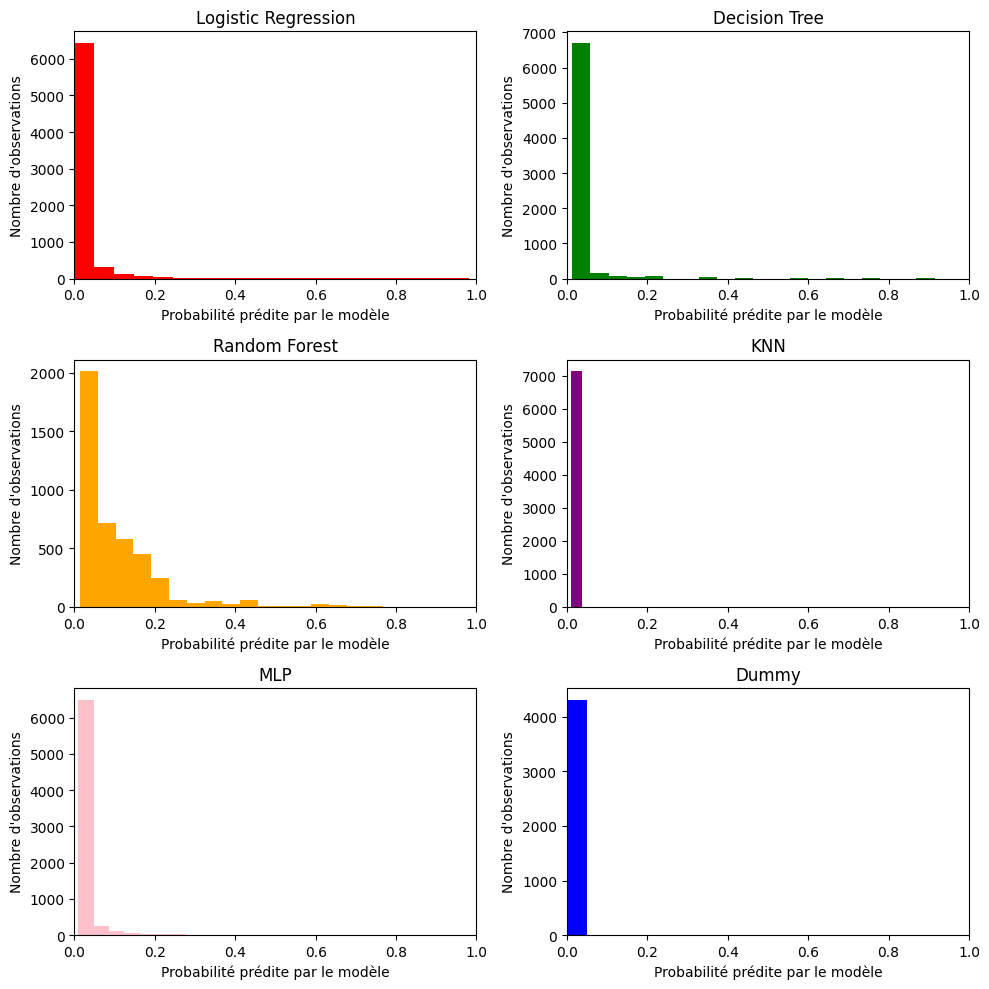
\includegraphics[width=\textwidth]{img/distributions_result_from_models.png}
    \caption{Distribution des résultats prédits sur les données de test}
    \label{fig:results}
\end{figure}

\newpage

\subsection{Visualisation des résultats sur un terrain}
Pour ajouter une nouvelle manière d'analyser et visualiser les résultats, nous avons décidé de créer une heatmap pour chacune des positions du terrains de football.
À partir de cela, nous calculerons la distance et l'angle. 
Nous avons également indiqué que tous les tirs effectués à chacune des positions n'ont pas été effectués de la tête et qu'ils ont été effectués avec le pied fort du joueur.
Nous sommes amenés à voir que la majorité des tirs ont été effectués avec le pied fort du joueur et qu'ils n'ont pas été effectués de la tête (voir figure \ref{fig:analyse_qualitative}).
Il est donc plus pertinent, pour cette visualisation, de se concentrer sur la position du tir pour éviter d'ajouter un éventuel biais à notre visualisation en prenant uniquement en compte les tirs du pied faible ou de la tête.

\begin{figure}[htp]
    \centering
    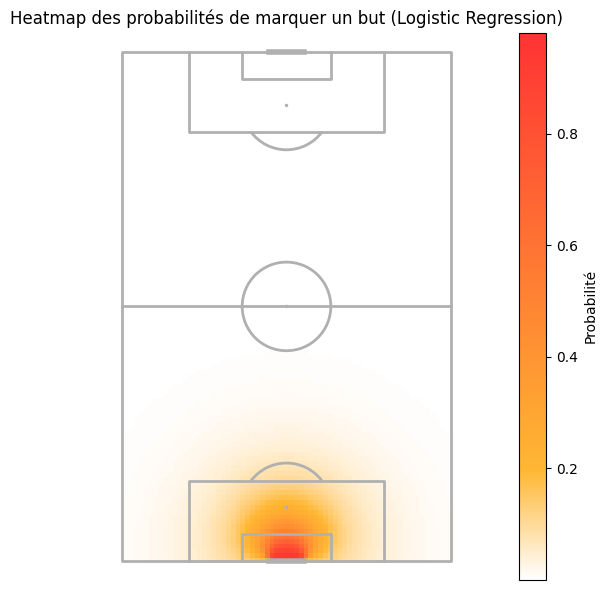
\includegraphics[width=0.7\textwidth]{img/pitch_visualisation_log_reg.png}
    \caption{Heatmap des résultats prédits par la régression logistique}
    \label{fig:result_log_reg}
\end{figure}

\begin{figure}[htp]
    \centering
    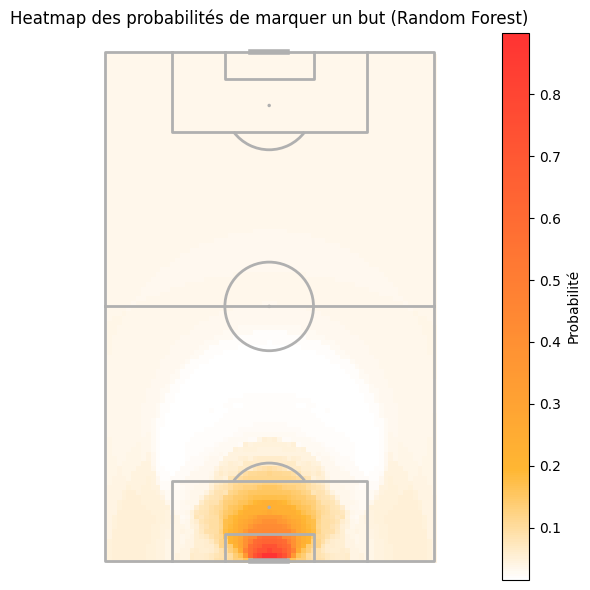
\includegraphics[width=0.6\textwidth]{img/pitch_visualisation_random_forest.png}
    \caption{Heatmap des résultats prédits par le modèle Random Forest}
    \label{fig:result_random_forest}
\end{figure}

\begin{figure}[htp]
    \centering
    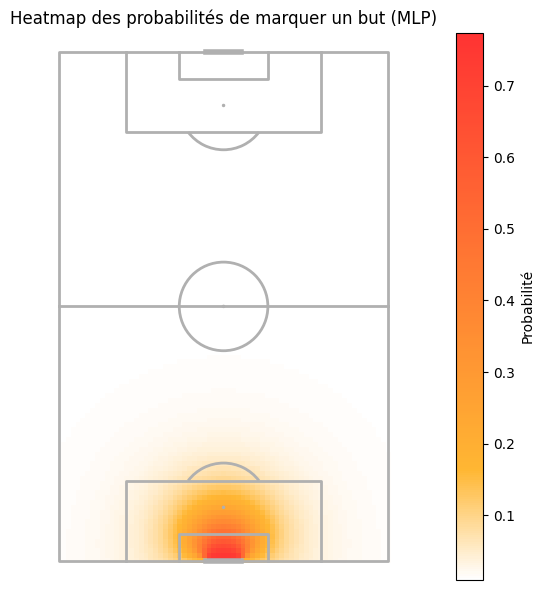
\includegraphics[width=0.6\textwidth]{img/pitch_visualisation_mlp.png}
    \caption{Heatmap des résultats prédits par le perceptron multi-couches}
    \label{fig:result_mlp}
\end{figure}

\begin{figure}[htp]
    \centering
    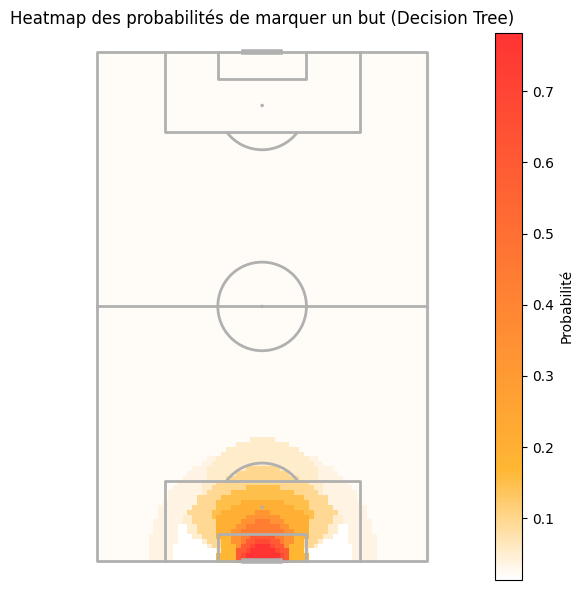
\includegraphics[width=0.6\textwidth]{img/pitch_visualisation_tree.png}
    \caption{Heatmap des résultats prédits par l'arbre de décision}
    \label{fig:result_tree}
\end{figure}

\begin{figure}[htp]
    \centering
    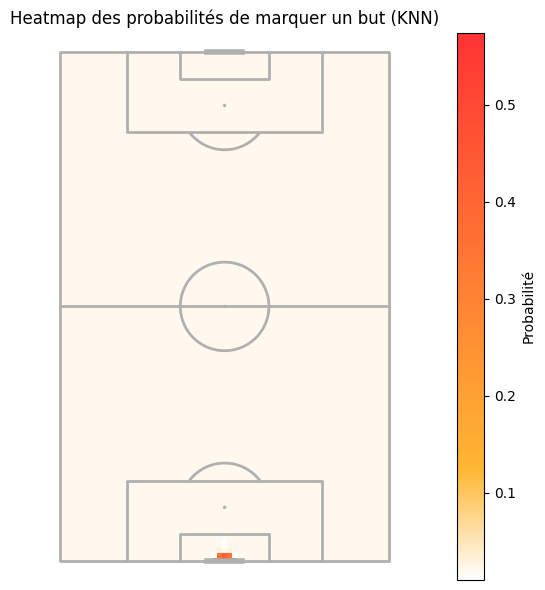
\includegraphics[width=0.5\textwidth]{img/pitch_visualisation_knn.png}
    \caption{Heatmap des résultats prédits par le modèle KNN}
    \label{fig:result_knn}
\end{figure}
\newpage
Lorsque nous nous penchons sur les figures \ref{fig:result_log_reg}, \ref{fig:result_random_forest}, \ref{fig:result_mlp}, \ref{fig:result_tree}, nous constatons que la tendance générale des modèles est la même.
C'est-à-dire qu'ils prédisent que les tirs effectués dans la surface de réparation ont une plus grande chance d'être transformés en but que ceux effectués à l'extérieur de la surface.
Cependant, nous pouvons constater plusieurs phénomènes.
Tout d'abord, nous nous apercevons que le modèle Random Forest prédit que les tirs effectués du côté du terrain de l'équipe attaquante ont une plus grande chance d'être marqués que ceux qui sont effectués à l'extérieur de la surface mais dans le camp adverse.
C'est également visible pour l'arbre de décision qui prédit une plus forte chance de marquer pour les tirs effectués dans le propre camp que ceux effectués dans la surface adverse dans un angle relativement faible.
Ce phénomène peut être dû à un manque de tirs faits à très longue distance des modèles.
En effet, lorsque nous observons la figure \ref{fig:pitch_chart}, nous constatons que les tirs sont majoritairement effectués dans la surface de réparation adverse et dans le camp adverse.
Cela explique pourquoi ces deux modèles ont une bonne prédiction lorsque le tir est effectué dans ces zones.
Cependant, nous pouvons voir que les tirs effectués dans le propre camp sont très peu nombreux.
L'hypothèse est que ces modèles ont bien appris sur la majorité des tirs, mais que le manque de tirs effectués dans le propre camp a fait que ces deux modèles ont eu plus de difficultés à effectuer des prédictions correctes pour ces tirs.
\newline\newline
Ensuite, nous pouvons voir que le modèle KNN prédit de manière incorrecte les probabilités.
Nous avons été en mesure de le voir via sa log loss qui était relativement élevée par rapport aux autres modèles.
Nous pouvons également le voir sur la figure \ref{fig:result_knn} où nous constatons que les probabilités prédites sont très similaires pour toutes les positions du terrain, sauf pour les tirs effectués à 1 mètre du but adverse.
\newline\newline
C'est alors via ces visualisations que nous pouvons constater et comparer les différences entre les modèles.
Nous nous apercevons que les deux modèles les plus performants sont la régression logistique et le perceptron multi-couches.
La régression logistique a une meilleure log loss que le perceptron multi-couches.
Nous voyons notamment que malgré le fait que la log loss du perceptron multi-couches soit plus élevée que le modèle Random Forest, sa visualisation en heatmap est plus proche de la réalité que le modèle Random Forest qui lui fournit des résultats incohérents à très longue distance.
Nous avons vu via la tendance des prédictions des modèles que la chance de réussite d'un tir augmente plus le tir est effectué proche du but adverse.
Sur la figure \ref{fig:pitch_chart}, nous voyons que les joueurs professionnels de football ont déjà connaissance que leurs chances de tirs augmentent plus ils sont proches du but adverse.
\newline\newline
Pour conclure cette section sur l'analyse des résultats, nous pouvons dire que la régression logistique est le modèle le plus performant pour résoudre ce problème. 
Il est important de rappeler qu'uniquement 5 modèles de classifications ont été testés.
Dû à un manque de puissance de calcul, il n'a pas été possible de tester plus de modèles, ni de fournir davantage d'hyper paramètres.
Il est donc possible qu'un autre modèle soit plus performant que la régression logistique pour la résolution de ce cas.
\newpage
\section{Conclusion}

\subsection{Conclusion générale}
Nous allons maintenant nous pencher sur la conclusion finale de ce travail.
Tout d'abord, nous allons nous pencher sur la première question du travail qui était de savoir quels étaient les facteurs qui influençaient le plus la réussite d'un tir.
Via nos recherches sur le sujet, nous avons pu établir un état de l'art sur le sujet.
Nous avons pu observer, via cet état de l'art, que les facteurs les plus influents étaient la distance du tir ainsi que l'angle du tir.
Ils sont d'ailleurs indissociables puisque le cumul des deux apporte une information plus pertinente que chacun des deux facteurs pris séparément.
L'un des articles scientifiques a également essayé d'introduire un facteur supplémentaire indiquant si le tir a été effectué de la tête.
Cependant, rien est indiqué si ce facteur a une réelle influence sur la réussite d'un tir.
\newline\newline
Dans notre travail, nous avons pu constater et confirmer que la distance et l'angle du tir étaient les facteurs les plus influents.
En effet, ces deux facteurs sont corrélés (voir fig. \ref{fig:analyse_quantitative}) et ont une réelle influence sur la réussite d'un tir.
Nous avons fait le travail de sélection des meilleurs attributs pour nos modèles dans la section \ref{sec:selection_attributs}. 
Cette recherche a consisté à faire une "forward elimination" sur les attributs de notre dataset.
Le principe de cette méthode est de commencer avec un modèle vide et d'ajouter un attribut à la fois.
Ensuite, nous observons si l'ajout de cet attribut améliore les performances du modèle.
Dans notre cas, nous observions si la p-value de l'attribut était inférieure à 0.05.
Si c'était le cas, nous gardions l'attribut et nous recommencions l'opération avec un autre attribut.
La p-value est une valeur qui indique si l'attribut est significatif pour le modèle.
Dans notre cas, ce test a été fait avec une régression logistique.
Lorsque la "forward elimination" a été faite, nous avons pu constater que les attributs les plus influents étaient :
\begin{itemize}
    \item La distance du tir
    \item L'angle du tir
    \item Si le tir a été effectué de la tête
    \item Si le tir a été effectué avec le pied fort du joueur
\end{itemize}
Nous pouvons d'ailleurs le voir sur le tableau \ref{tab:logistic_regression_result_6}.
Ce dernier affiche les résultats de la régression logistique avec les attributs sélectionnés. 
On peut y observer les p-values de chaque attribut ainsi que leurs coefficients.
C'est donc ainsi que nous avons pu répondre à la première question de ce travail.
\newline\newline
Ensuite, nous avons pu répondre à la deuxième question de ce travail qui était de savoir quel modèle est le plus performant pour résoudre ce problème.
Pour répondre à cette question, il a fallu établir une bonne méthodologie.
\newline\newline
Dans notre cas, nous avons décidé de faire une séparation du dataset en deux parties.
La première partie était utilisée pour l'entraînement des modèles et la deuxième partie était utilisée pour tester les modèles.
L'entraînement des modèles consistait à faire une validation croisée avec 5 folds pour trouver les meilleurs hyper paramètres pour chaque modèle.
Ensuite, nous avons pu tester les modèles avec leurs meilleurs hyper paramètres trouvés sur la deuxième partie du dataset.
\newline\newline
Les résultats sur la deuxième partie du dataset nous ont permis de comparer les modèles entre eux.
Nous les avons comparé via la log loss et via la visualisation des probabilités prédites par les modèles.
Nous avons pu constater des choses intéressantes sur les résultats.
Tout d'abord, nous avons pu constater, via le tableau \ref{tab:results}, que les 3 modèles les plus performants selon la log loss étaient la régression logistique, le modèle Random Forest et le perceptron multi-couches.
Cependant, après avoir visualisé les probabilités prédites par les modèles sur un terrain de football, nous avons pu constater que le modèle Random Forest fournissait des résultats incohérents à longue distance (voir fig. \ref{fig:result_random_forest}).
Les deux autres modèles précédemment cités fournissaient des résultats plus cohérents par rapport à la réalité (voir fig. \ref{fig:result_log_reg} et \ref{fig:result_mlp}).
\newline\newline
Pour finir, nous pouvons dire que la régression logistique est le modèle le plus performant pour résoudre ce problème de prédiction de la réussite d'un tir.
Ce modèle est utilisé avec la distance, l'angle, l'information du tir effectué de la tête et du pied fort.
\newpage

\subsection{Améliorations possibles}
En termes d'améliorations possibles, nous pouvons dire que ce travail peut être amélioré de plusieurs manières.
Tout d'abord, nous pourrions améliorer ajouter de nouveaux attributs.
En effet, nous pourrions ajouter davantage de données pour apporter des détails supplémentaires sur le tir.
Par exemple, il serait intéressant d'ajouter la hauteur du ballon au moment du tir, le type d'attaque effectuée (contre-attaque, attaque placée, etc.), le type de passe effectuée (passe en profondeur, passe en retrait, etc.), ou encore ajouter des informations quant à la qualité du joueur à terminer les actions.
Effectivement, un défenseur a, en théorie, une moins bonne qualité de finition qu'un attaquant. 
Cette différenciation pourrait également se faire entre les différents attaquants. 
Par exemple, Cristiano Ronaldo a la capacité de marquer plus de buts dans des situations difficiles qu'un attaquant de Ligue 2.
Il serait également envisageable d'ajouter le même type d'informations pour le gardien de but.
\newline\newline
Ensuite, nous pourrions tester et comparer d'autres modèles non testés ici.
Par exemple, nous pourrions tester un modèle de classification basée sur SVM.
Finalement, nous pourrions également expérimenter d'ajouter de nouveaux hyper paramètres pour les modèles testés.
En effet, dû à un manque de puissance de calcul et de temps, nous n'avons pas pu tester tous les hyper paramètres possibles pour chaque modèle.
\newpage

% Bibliography
\bibliographystyle{plain}
\bibliography{bibliography}

\end{document}